\documentclass[10pt,a4paper]{article}
\usepackage[UTF8,fontset = windows]{ctex}
\setCJKmainfont[BoldFont=黑体,ItalicFont=楷体]{华文中宋}
\usepackage{amssymb,amsmath,amsfonts,amsthm,mathrsfs,dsfont,graphicx}
\usepackage{ifthen,indentfirst,enumerate,color,titletoc}
\usepackage{tikz}
\usetikzlibrary{arrows,calc}
\usepackage[bf,small,indentafter,pagestyles]{titlesec}
\usepackage[top=1in, bottom=1in,left=0.8in,right=0.8in]{geometry}
\renewcommand{\baselinestretch}{1.65}
\newtheorem{defi}{定义~}
\newtheorem{eg}{例~}
\newtheorem{ex}{~}
\newtheorem{rem}{注~}
\newtheorem{thm}{定理~}
\newtheorem{coro}{推论~}
\newtheorem{axiom}{公理~}
\newtheorem{prop}{性质~}

\newcommand{\blank}[1]{\underline{\hbox to #1pt{}}}
\newcommand{\bracket}[1]{(\hbox to #1pt{})}

\begin{document}

\begin{enumerate}[1.]

%赋能1

\item  若``$a>b$'', 则``$a^3>b^3$''是\blank{50}命题(填: 真、假).
\item  已知$A=(-\infty ,0]$, $B=(a,+\infty )$, 若$A\cup B=\mathbf{R}$, 则$a$的取值范围是\blank{50}.
\item  $z+2\bar{z}=9+4\mathrm{i}$($\mathrm{i}$为虚数单位), 则$|z|=$\blank{50}.
\item  若$\triangle ABC$中, $a+b=4$, $\angle C=30^\circ$, 则$\triangle ABC$面积的最大值是\blank{50}.
\item  若函数$f(x)=\log_2\dfrac{x-a}{x+1}$的反函数的图像过点$(-2,3)$, 则$a=$\blank{50}.
\item  若半径为2的球$O$表面上一点$A$作球$O$的截面, 若$OA$与该截面所成的角是$60^\circ$, 则该
截面的面积是\blank{50}.
\item  抛掷一枚均匀的骰子(刻有1、2、3、4、5、6)三次, 得到的数字依次记作$a$、$b$、$c$, 则$a+b\mathrm{i}$($\mathrm{i}$为虚数单位)是方程$x^2-2x+c=0$的根的概率是\blank{50}.
\item  设常数$a>0$, $(x+\dfrac{a}{\sqrt{x}})^9$展开式中$x^6$的系数为$4$, 则$\displaystyle\lim_{n\to \infty}(a+a^2+\cdots+a^n)=$\blank{50}.
\item  已知直线$l$经过点$(-\sqrt{5},0)$且方向向量为$(2,-1)$, 则原点$O$到直线$l$的距离为\blank{50}.
\item  若双曲线的一条渐近线为$x+2y=0$, 且双曲线与抛物线$y=x^2$的准线仅有一个公共点, 则此双曲线的标准方程为\blank{50}.

%赋能2

\item $\displaystyle\lim_{n\to \infty}\dfrac{2n-5}{n+1}=$\blank{50}.
\item 已知抛物线$C$的顶点在平面直角坐标系原点, 焦点在$x$轴上, 若$C$经过点$M(1,3)$, 则其焦点到准线的距离为\blank{50}.
\item 若线性方程组的增广矩阵为$\begin{pmatrix}    a & 0 & 2 \\ 0 & 1 & b\end{pmatrix}$, 解为$\begin{cases}    x=2, \\ y=1.\end{cases}$ 则$a+b=$\blank{50}.
\item 若复数$z$满足: $\mathrm{i}\cdot z=\sqrt{3}+\mathrm{i}$($\mathrm{i}$是虚数单位), 则$|z|=$\blank{50}.
\item 在$(x+\dfrac{2}{x^2})^6$的二项展开式中第四项的系数是\blank{50}(结果用数值表示).
\item 在长方体$ABCD-A_1B_1C_1D_1$中, 若$AB=BC=1$, $AA_1=\sqrt{2}$, 则异面直线$BD_1$与$CC_1$所成角的大小为\blank{50}.
\item 若函数$f(x)=\begin{cases}    2^x, & x\le 0, \\ -x^2+m, & x>0 \end{cases}$的值域为$(-\infty ,1]$, 则实数$m$的取值范围是\blank{50}.
\item 如图, 在$\triangle ABC$中, 若$AB=AC=3$, $\cos \angle BAC=\dfrac{1}{2}$, $\overrightarrow{DC}=2\overrightarrow{BD}$, 则$\overrightarrow{AD}\cdot \overrightarrow{BC}=$\blank{50}.
\begin{center}
    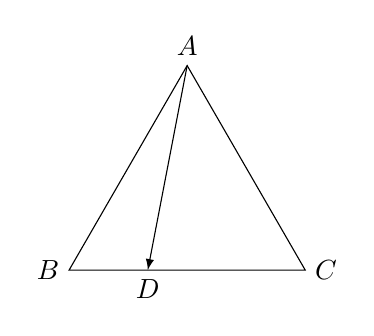
\begin{tikzpicture}[>=latex]
        \draw (0,0) node [left] {$B$} -- (3,0) node [right] {$C$} -- (1.5,{1.5*sqrt(3)}) node [above] {$A$} coordinate (A) -- cycle;
        \draw [->] (A) -- (1,0) node [below] {$D$};
    \end{tikzpicture}
\end{center}
\item 定义在$\mathbf{R}$上的偶函数$y=f(x)$, 当$x\ge 0$时, $f(x)=\lg (x^2-3x+3)$, 则$f(x)$在$\mathbf{R}$上的零点个数为\blank{50}个.
\item 将$6$辆不同的小汽车和$2$辆不同的卡车驶入如图所示的$10$个车位中的某$8$个内, 其中$2$辆卡车必须停在$A$与$B$的位置, 那么不同的停车位置安排共有\blank{50}种(结果用数值表示).
\begin{center}
    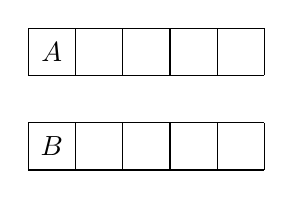
\begin{tikzpicture}[>=latex]
        \draw (0,0) node {$B$};
        \draw (0,1.2) node {$A$};
        \foreach \i in {-0.3,0.3,0.9,1.5}{\draw (-0.3,\i) -- (2.7,\i);};
        \foreach \i in {-0.3,0.3,...,2.8}{\draw (\i,-0.3) -- (\i, 0.3) (\i, 0.9) -- (\i, 1.5);};
    \end{tikzpicture}
\end{center}

% 赋能3 

\item 设集合$A=\{x||x-2|<1,x\in \mathbf{R}\}$, 集合$B=\mathbf{Z}$, 则$A\cap B=$\blank{50}.
\item 函数$y=\sin (\omega x-\dfrac{\pi}{3})$($\omega >0$)的最小正周期是$\pi$, 则$\omega =$\blank{50}.
\item 设$\mathrm{i}$为虚数单位, 在复平面上, 复数$\dfrac{3}{(2-\mathrm{i})^2}$对应的点到原点的距离为\blank{50}.
\item 若函数$f(x)=\log_2 (x+1)+a$的反函数的图像经过点$(4,1)$, 则实数$a=$\blank{50}.
\item 已知$(a+3b)^n$的展开式中, 各项系数的和与各项二项式系数的和之比为$64$, 则$n=$\blank{50}.
\item 甲、乙两人从$5$门不同的选修课中各选修$2$门, 则甲、乙所选的课程中恰有$1$门相同的选法有\blank{50}种.
\item 若圆锥的侧面展开图是半径为2$\text{cm}$, 圆心角为$270^\circ$的扇形, 则这个圆锥的体积为\blank{50}$\text{cm}^3$.
\item 若数列$\{a_n\}$的所有项都是正数, 且$\sqrt{a_1}+\sqrt{a_2}+\cdots +\sqrt{a_n}=n^2+3n$($n\in \mathbf{N}^*$), 则$\displaystyle\lim_{n\to\infty}\dfrac{1}{n^2}(\dfrac{a_1}{2}+\dfrac{a_2}{3}+\cdots +\dfrac{a_n}{n+1})=$\blank{50}.
\item 如图, 在$\triangle ABC$中, $\angle B=45^\circ$, $D$是$BC$边上的一点, $AD=5$, $AC=7$, $DC=3$, 则$AB$的长为\blank{50}.
\begin{center}
    \begin{tikzpicture}[scale = 0.5]
        \draw  (-6.830127018922193,0.)-- (3.,0.) node [below right] {$C$};
        \draw  (3.,0.)-- (-2.5,4.330127018922193) node [above] {$A$};
        \draw  (-2.5,4.330127018922193)-- (-6.830127018922193,0.) node [below left] {$B$};
        \draw  (-2.5,4.330127018922193)-- (0.,0.) node [below] {$D$};
    \end{tikzpicture}
\end{center}
\item 有以下命题:\\
\textcircled{1} 若函数$f(x)$既是奇函数又是偶函数, 则$f(x)$的值域为$\{0\}$; \\
\textcircled{2} 若函数$f(x)$是偶函数, 则$f(|x|)=f(x)$;\\
\textcircled{3} 若函数$f(x)$在其定义域内不是单调函数, 则$f(x)$不存在反函数;\\
\textcircled{4} 若函数$f(x)$存在反函数${{f}^{-1}}(x)$, 且${{f}^{-1}}(x)$与$f(x)$不完全相同, 则$f(x)$与${{f}^{-1}}(x)$图像的公共点必在直线$y=x$上; \\
其中真命题的序号是\blank{50}(写出所有真命题的序号).

% 赋能4

\item 若集合$A=\{x|y^2=x,y\in \mathbf{R}\}$, $B=\{y|y=\sin x,x\in \mathbf{R}\}$, 则$A\cap B=$\blank{50}.
\item 若$-\dfrac{\pi}{2}<\alpha <\dfrac{\pi}{2}$, $\sin \alpha =\dfrac{3}{5}$, 则$\cot 2\alpha =$\blank{50}.
\item 函数$f(x)=1+\log_2 x$($x\ge 1$)的反函数$f^{-1}(x)=$\blank{50}.
\item 若$(1+x)^5=a_0+a_1x+a_2x^2+\cdots+a_5x^5$, 则$a_1+a_2+\cdots+a_5=$\blank{50}.
\item 设$k\in \mathbf{R}$, $\dfrac{y^2}{k}-\dfrac{x^2}{k-2}=1$表示焦点在$y$轴上的双曲线, 则半焦距的取值范围是\blank{50}.
\item 设$m\in \mathbf{R}$, 若$f(x)=(m+1)x^{\tfrac{2}{3}}+mx+1$是偶函数, 则$f(x)$的单调递增区间是\blank{50}.
\item 方程$\log_2(9^x-5)=2+\log_2(3^x-2)$的解$x=$\blank{50}.
\item 已知圆$C:x^2+y^2+2kx+2y+k^2=0$($k\in \mathbf{R}$)和定点$P(1,-1)$, 若过$P$可以作两条直线与圆$C$相切, 则$k$的取值范围是\blank{50}.
\item 如图, 在直三棱柱$ABC-A_1B_1C_1$中, $\angle ABC=90^\circ$, $AB=BC=1$, 若$A_1C$与平面$B_1BCC_1$所成的角为$\dfrac{\pi}{6}$, 则三棱锥$A_1-ABC$的体积为\blank{50}.
\begin{center}
    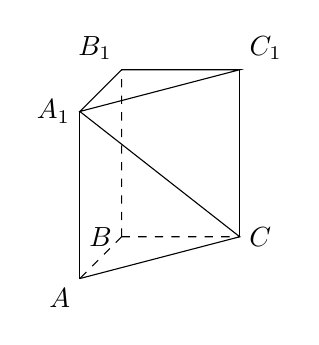
\begin{tikzpicture}[scale = 1.5]
        \draw [dashed] (0,0) -- (1,0) node [right] {$C$} coordinate (C) (0,0) -- (225:0.5) node [below left] {$A$} coordinate (A) (0,0) node [left] {$B$} coordinate (B) -- (0,{sqrt(2)}) node [above left] {$B_1$} coordinate (B1);
        \draw (A) --+ (0,{sqrt(2)}) node [left] {$A_1$} coordinate (A1);
        \draw (C) --+ (0,{sqrt(2)}) node [above right] {$C_1$} coordinate (C1);
        \draw (A1) -- (B1) -- (C1) -- (A1) -- (C) -- (A);
    \end{tikzpicture}
\end{center}
\item 设地球半径为$R$, 若$A$、$B$两地均位于北纬$45^\circ$, 且两地所在纬度圈上的弧长为$\dfrac{\sqrt{2}}{4}\pi R$, 则$A$、$B$之间的球面距离是\blank{50}(结果用含有$R$的代数式表示).

% 赋能5

\item 复数$\mathrm{i}(2+\mathrm{i})$的虚部为\blank{50}.
\item 设函数$f(x)=\begin{cases}\log_2 x, & x>0, \\ 4^x, & x\le 0,\end{cases}$ 则$f(f(-1))=$\blank{50}.
\item 已知$M=\{x||x-1|\le 2,x\in \mathbf{R}\}$, $P=\{x|\dfrac{1-x}{x+2}\ge 0,x\in \mathbf{R}\}$, 则$M\cap P=$\blank{50}.
\item 抛物线$y=x^2$上一点$M$到焦点的距离为$1$, 则点$M$的纵坐标为\blank{50}.
\item 已知无穷数列$\{a_n\}$满足$a_{n+1}=\dfrac12{a_n}$($n\in \mathbf{N}^*$), 且$a_2=1$, 记$S_n$为数列$\{a_n\}$的前$n$项和, 则$\displaystyle\lim_{n\to \infty}S_n=$\blank{50}.
\item 已知$x,y\in \mathbf{R}^+$, 且$x+2y=1$, 则$xy$的最大值为\blank{50}.
\item 已知圆锥的母线$l=10$, 母线与旋转轴的夹角$\alpha =30^\circ$, 则圆锥的表面积为\blank{50}.
\item 若$(2x^2+\dfrac1x)^n$($n\in \mathbf{N}^*$)的二项展开式中的第$9$项是常数项, 则$n=$\blank{50}.
\item 已知$A,B$分别是函数$f(x)=2\sin \omega x$($\omega >0$)在$y$轴右侧图像上的第一个最高点和第一个最低点, 且$\angle AOB=\dfrac\pi 2$, 则该函数的最小正周期是\blank{50}.
\item 将序号分别为1、2、3、4、5的$5$张参观券全部分给$4$人, 每人至少一张, 如果分给同一人的$2$张参观券连号, 那么不同的分法种数是\blank{50}.

% 赋能6

\item $\displaystyle\lim_{n\to\infty}\dfrac{2n+3}{n+1}=$\blank{50}.
\item 设全集$U=\mathbf{R}$, 集合$A=\{-1,0,1,2,3\}$, $B=\{x|x\ge 2\}$, 则$A\cap {\complement_U}B=$\blank{50}.
\item 不等式$\dfrac{x+1}{x+2}<0$的解集为\blank{50}.
\item 椭圆$\begin{cases} x=5\cos \theta,  \\ y=4\sin \theta  \end{cases}$($\theta$为参数)的焦距为\blank{50}.
\item 若函数$y=\begin{vmatrix}   \cos x & \sin x  \\   \sin x & \cos x  \\ \end{vmatrix}$的最小正周期为$a\pi $, 则实数$a$的值为\blank{50}.
\item 若点$(8,4)$在函数$f(x)=1+\log_a x$图像上, 则$f(x)$的反函数为\blank{50}.
\item 已知向量$\overrightarrow{a}=(1,2)$, $\overrightarrow{b}=(0,3)$, 则$\overrightarrow{b}$在$\overrightarrow{a}$的方向上的投影为\blank{50}.
\item 已知一个底面置于水平面上的圆锥, 其左视图是边长为6的正三角形, 则该圆锥的侧面积为\blank{50}.
\item 某班级要从$5$名男生和$2$名女生中选出$3$人参加公益活动, 则在选出的$3$人中男、女生
均有的概率为\blank{50}(结果用最简分数表示).
\item 设常数$a>0$, 若$(x+\dfrac ax)^9$的二项展开式中$x^5$的系数为$144$, 则$a=$\blank{50}.

% 赋能7

\item 设集合$M=\{x|x^2=x\}$, $N=\{x|\lg x\le 0\}$, 则$M\cap N=$\blank{50}.
\item 已知$a$、$b\in \mathbf{R}$, $\mathrm{i}$是虚数单位, 若$a+\mathrm{i}=2-b\mathrm{i}$, 则$(a+b\mathrm{i})^2=$\blank{50}.
\item 已知函数$f(x)=a^x-1$的图像经过$(1,1)$点, 则$f^{-1}(3)=$\blank{50}.
\item 不等式$x|x-1|>0$的解集为\blank{50}.
\item 已知$\overrightarrow a=(\sin x,\cos x)$, $\overrightarrow b=(\sin x,\sin x)$, 则函数$f(x)=\overrightarrow a\cdot \overrightarrow b$的最小正周期为\blank{50}.
\item 里约奥运会游泳小组赛采用抽签方法决定运动员比赛的泳道, 在由$2$名中国运动员和$6$名外国运动员组成的小组中, $2$名中国运动员恰好抽在相邻泳道的概率为\blank{50}.
\item 如图, 在棱长为$1$的正方体$ABCD-A_1B_1C_1D_1$中, 点$P$在截面$A_1DB$上, 则线段$AP$的最小值为\blank{50}.
\begin{center}
    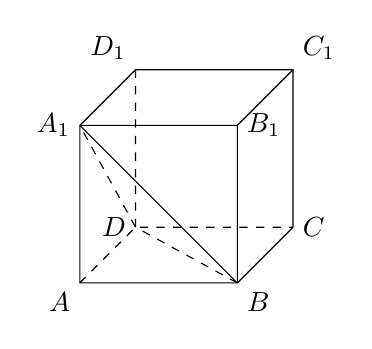
\begin{tikzpicture}
        \draw (0,0) node [below left] {$A$} coordinate (A) --++ (2,0) node [below right] {$B$} coordinate (B) --++ (45:{2/2}) node [right] {$C$} coordinate (C)
        --++ (0,2) node [above right] {$C_1$} coordinate (C1)
        --++ (-2,0) node [above left] {$D_1$} coordinate (D1) --++ (225:{2/2}) node [left] {$A_1$} coordinate (A1) -- cycle;
        \draw (A) ++ (2,2) node [right] {$B_1$} coordinate (B1) -- (B) (B1) --++ (45:{2/2}) (B1) --++ (-2,0);
        \draw [dashed] (A) --++ (45:{2/2}) node [left] {$D$} coordinate (D) --++ (2,0) (D) --++ (0,2);
        \draw (A1) -- (B);
        \draw [dashed] (B) -- (D) -- (A1);
    \end{tikzpicture}
\end{center}
\item 设$(1+x)^n=a_0+a_1x+a_2x^2+a_3x^3+\cdots +a_nx^n$, 若$\dfrac{a_2}{a_3}=\dfrac13$, 则$n=$\blank{50}.
\item 已知圆锥底面半径与球的半径都是$1\text{cm}$, 如果圆锥的体积与球的体积恰好也相等, 那么这个圆锥的侧面积是\blank{50}$\text{cm}^2$.
\item 设$P(x,y)$是曲线$C:\sqrt{\dfrac{x^2}{25}}+\sqrt{\dfrac{y^2}9}=1$上的点, $F_1(-4,0)$, $F_2(4,0)$, 则$|PF_1|+|PF_2|$的最大值为\blank{50}.

% 赋能8

\item 已知复数$z=2+\mathrm{i}$($\mathrm{i}$为虚数单位), 则$\overline{{z^2}}=$\blank{50}.
\item 已知集合$A=\{x|\dfrac12\le {2^x}<16\}$, $B=\{x|y=\log _2(9-x^2)\}$, 则$A\cap B=$\blank{50}.
\item 在二项式$(x+\dfrac2x)^6$的展开式中, 常数项是\blank{50}.
\item 等轴双曲线$x^2-y^2=a^2$与抛物线$y^2=16x$的准线交于$A$、$B$两点, 且$|AB|=4\sqrt3$, 则该双曲线的实轴长等于\blank{50}.
\item 若由矩阵$\begin{pmatrix}a & 2 \\ 2 & a\end{pmatrix}\begin{pmatrix}x \\ y\end{pmatrix}=\begin{pmatrix}a+2 \\ 2a\end{pmatrix}$表示$x$、$y$的二元一次方程组无解, 则实数$a=$\blank{50}.
\item 已知$f(x)=\sin\dfrac\pi 3x$, $A=\{1,2,3,4,5,6,7,8\}$, 现从集合$A$中任取两个不同元素$s$、$t$, 则使得$f(s)\cdot f(t)=0$发生的概率是\blank{50}.
\item 若圆锥侧面积为$20\pi$, 且母线与底面所成角为$\arccos \dfrac45$, 则该圆锥的体积为\blank{50}.
\item 已知数列$\{a_n\}$的通项公式为$a_n=n^2+bn$, 若数列$\{a_n\}$是单调递增数列, 则实数$b$的取值范围是\blank{50}.
\item 将边长为$10$的正三角形$ABC$, 按``斜二测''画法在水平放置的平面上画出为$\triangle A'B'C'$, 则$\triangle A'B'C'$中最短边的边长为\blank{50}(精确到0.01).
\item 已知点$A$是圆$O: x^2+y^2=4$上的一个定点, 点$B$是圆$O$上的一个动点, 若满足$|\overrightarrow{AO}+\overrightarrow{BO}|=|\overrightarrow{AO}-\overrightarrow{BO}|$, 则$\overrightarrow{AO}\cdot \overrightarrow{AB}=$\blank{50}.

% 赋能9

\item 方程$\lg (3x+4)=1$的解$x=$\blank{50}.
\item 若关于$x$的不等式$\dfrac{x-a}{x-b}>0$($a,b\in \mathbf{R}$)的解集为$(-\infty ,1)\cup (4,+\infty)$, 则$a+b=$\blank{50}.
\item 已知数列$\{a_n\}$的前$n$项和为$S_n=2^n-1$, 则此数列的通项公式为\blank{50}.
\item 函数$f(x)=\sqrt x+1$的反函数是\blank{50}.
\item $(1+2x)^6$展开式中$x^3$项的系数为\blank{50}(用数字作答).
\item 如图, 已知正方形$ABCD-A_1B_1C_1D_1$, $AA_1=2$, $E$为棱$CC_1$的中点, 则三棱锥$D_1-ADE$的体积为\blank{50}.
\begin{center}
    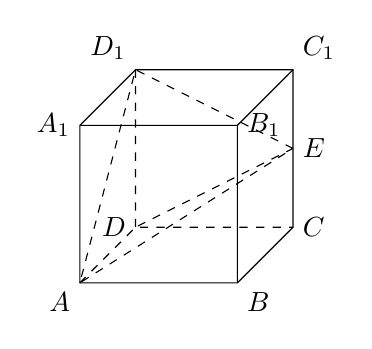
\begin{tikzpicture}
        \draw (0,0) node [below left] {$A$} coordinate (A) --++ (2,0) node [below right] {$B$} coordinate (B) --++ (45:{2/2}) node [right] {$C$} coordinate (C)
        --++ (0,2) node [above right] {$C_1$} coordinate (C1)
        --++ (-2,0) node [above left] {$D_1$} coordinate (D1) --++ (225:{2/2}) node [left] {$A_1$} coordinate (A1) -- cycle;
        \draw (A) ++ (2,2) node [right] {$B_1$} coordinate (B1) -- (B) (B1) --++ (45:{2/2}) (B1) --++ (-2,0);
        \draw [dashed] (A) --++ (45:{2/2}) node [left] {$D$} coordinate (D) --++ (2,0) (D) --++ (0,2);
        \draw ($ (C)!0.5!(C1) $) node [right] {$E$} coordinate (E);
        \draw [dashed] (E) -- (D1) -- (A) -- (E) -- (D);
    \end{tikzpicture}
\end{center}
\item 从单词``shadow''中任意选取$4$个不同的字母排成一排, 则其中含有``a''的共有\blank{50}种排法(用数字作答).
\item 集合$\{x|\cos (\pi \cos x)=0,x\in [0,\pi]\}=$\blank{50}(用列举法表示).
\item 如图, 已知半径为1的扇形$AOB$, $\angle AOB=60^\circ$, $P$为弧$\overset\frown{AB}$上的一个动点, 则$\overrightarrow{OP}\cdot \overrightarrow{AB}$取值范围是\blank{50}.
\begin{center}
    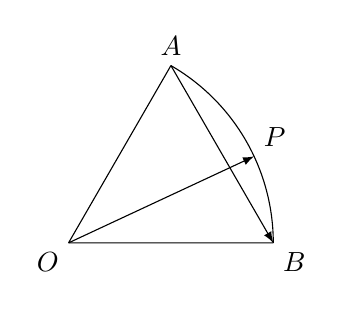
\begin{tikzpicture}[>=latex,scale = 1.3]
        \draw (0,0) node [below left] {$O$} -- (2,0) node [below right] {$B$} (0,0) -- (1,{sqrt(3)}) node [above] {$A$} -- cycle;
        \draw (2,0) arc (0:60:2);
        \draw [->] (0,0) -- (25:2) node [above right] {$P$};
        \draw [->] (1,{sqrt(3)}) -- (2,0);
    \end{tikzpicture}
\end{center}
\item 已知$x$、$y$满足曲线方程$x^2+\dfrac1{y^2}=2$, 则$x^2+y^2$的取值范围是\blank{50}.

% 赋能10

\item 已知$U=\mathbf{R}$, 集合$A=\{x|4-2x\ge x+1\}$, 则${\complement_U}A=$\blank{50}.
\item 三阶行列式$\begin{vmatrix}   3 & -5 & 1 \\   2 & 3 & -6 \\   -7 & 2 & 4 \\ \end{vmatrix}$中元素$-5$的代数余子式的值为\blank{50}.
\item $(1-\dfrac x2)^8$的二项展开式中含$x^2$项的系数是\blank{50}.
\item 已知一个球的表面积为$16\pi$, 则它的体积为\blank{50}.
\item 一个袋子中共有$6$个球, 其中$4$个红色球, $2$个蓝色球, 这些球的质地和形状一样, 从中任意抽取$2$个球, 则所抽的球都是红色球的概率是\blank{50}.
\item 已知直线$l:x-y+b=0$被圆$C:x^2+y^2=25$所截得的弦长为$6$, 则$b=$\blank{50}.
\item 若复数$(1+a\mathrm{i})(2-\mathrm{i})$在复平面上所对应的点在直线$y=x$上, 则实数$a=$\blank{50}.
\item 函数$f(x)=(\sqrt3\sin x+\cos x)(\sqrt3\cos x-\sin x)$的最小正周期为\blank{50}.
\item 过双曲线$C:\dfrac{x^2}{a^2}-\dfrac{y^2}4=1$的右焦点$F$作一条垂直于$x$轴的垂线交双曲线$C$的两条渐近线于$A$、$B$两点, $O$为坐标原点, 则$\triangle OAB$的面积的最小值为\blank{50}.
\item 若关于$x$的不等式$|2^x-m|-\dfrac1{2^x}<0$在区间$[0,1]$内恒成立, 则实数$m$的范围\blank{50}.

% 赋能11

\item 已知集合$A=\{1,2,4,6,8\}$, $B=\{x|x=2k,k\in A\}$, 则$A\cap B=$\blank{50}.
\item 已知$\dfrac{\overline z}{1-\mathrm{i}}=2+\mathrm{i}$, 则复数$z$的虚部为\blank{50}.
\item 设函数$f(x)=\sin x-\cos x$, 且$f(a)=1$, 则$\sin 2a=$\blank{50}.
\item 已知二元一次方程$\begin{cases} {a_1}x+{b_1}y={c_1}, \\  {a_2}x+{b_2}y={c_2} \end{cases}$的增广矩阵是$\begin{pmatrix} 1 & -1 & 1 \\  1 & 1 & 3 \\ \end{pmatrix}$, 则此方程组的解是\blank{50}.
\item 数列$\{a_n\}$是首项为$1$, 公差为$2$的等差数列, $S_n$是它前$n$项和, 则$\displaystyle\lim_{n\to\infty}\dfrac{S_n}{a_n^2}=$\blank{50}.
\item 已知角$A$是$\triangle ABC$的内角, 则``$\cos A=\dfrac12$''是``$\sin A=\dfrac{\sqrt3}2$''的\blank{50}条件(填``充分非必要''、``必要非充分''、``充要条件''、``既非充分又非必要''之一).
\item 若双曲线$x^2-\dfrac{y^2}{b^2}=1$的一个焦点到其渐近线距离为$2\sqrt2$, 则该双曲线焦距等于\blank{50}.
\item 若正项等比数列$\{a_n\}$满足: $a_3+a_5=4$, 则$a_4$的最大值为\blank{50}.
\item 已知函数$f(x)=\sin (2x+\dfrac\pi 3)$在区间$[0,a]$(其中$a>0$)上单调递增, 则实数$a$的取值范围是\blank{50}.
\item 设函数$f(x)=\begin{cases}    x^6, & x\ge 1,  \\   -2x-1, & x\le -1, \end{cases}$ 则当$x\le -1$时, $f[f(x)]$表达式的展开式中含${x^2}$项的系数是\blank{50}.

% 赋能12

\item ``$x<0$''是``$x<a$''的充分非必要条件, 则$a$的取值范围是\blank{50}.
\item 函数$f(x)=1-3\sin ^2(x+\dfrac\pi 4)$的最小正周期为\blank{50}.
\item 若复数$z$为纯虚数, 且满足$(2-\mathrm{i})z=a+\mathrm{i}$($\mathrm{i}$为虚数单位), 则实数$a$的值为\blank{50}.
\item 二项式$(x^2+\dfrac 1x)^5$的展开式中, $x$的系数为\blank{50}.
\item 用半径$1$米的半圆形薄铁皮制作圆锥型无盖容器, 其容积为\blank{50}立方米.
\item 已知$\alpha$为锐角, 且$\cos (\alpha +\dfrac\pi 4)=\dfrac35$, 则$\sin \alpha =$\blank{50}.
\item 已知正四棱柱$ABCD-A_1B_1C_1D_1$, $AB=a$, $AA_1=2a$, $E$、$F$分别是棱$AD$、$CD$的中点,则异面直线$BC_1$与$EF$所成角是\blank{50}.
\item 在无穷等比数列$\{a_n\}$中, $\displaystyle\lim_{n\to\infty}(a_1+a_2+\cdots+a_n)=\dfrac12$, 则$a_1$的取值范围是\blank{50}.
\item 某班班会准备从含甲、乙的$6$名学生中选取$4$人发言, 要求甲、乙两人至少有一人参加, 那么不同的发言顺序有\blank{50}种.
\item 已知奇函数$f(x)$是定义在$\mathbf{R}$上的增函数, 数列$\{x_n\}$是一个公差为$2$的等差数列, 满足$f(x_7)+f(x_8)=0$, 则$x_{2017}$的值为\blank{50}.

% 赋能13

\item 若集合$M=\{x|{x^2}-2x<0\}$, $N=\{x||x|>1\}$, 则$M\cap N=$\blank{50}.
\item 若复数$\angle OFA+\angle OFB={180^\circ}$满足$2z+\overline z=3-2\mathrm{i}$, 其中$\mathrm{i}$为虚数单位, 则$z=$\blank{50}.
\item 如果$\sin \alpha =-\dfrac5{13}$, 且$\alpha$为第四象限角, 则$\tan \alpha$的值是\blank{50}.
\item 函数$f(x)=\begin{vmatrix}   \cos x & \sin x  \\    \sin x & \cos x \end{vmatrix}$的最小正周期是\blank{50}.
\item 函数$f(x)=2^x+m$的反函数为$y=f^{-1}(x)$, 且$y=f^{-1}(x)$的图像过点$Q(5,2)$, 那么$m=$\blank{50}.
\item 点$(1,0)$到双曲线$\dfrac{x^2}4-y^2=1$的渐近线的距离是\blank{50}.
\item 如果实数$x$、$y$满足$\begin{cases} 2x-y\le 0, \\ x+y\le 3, \\  x\ge 0, \\ \end{cases}$, 则$2x+y$的最大值是\blank{50}.
\item 从$5$名学生中任选$3$人分别担任语文、数学、英语课代表, 其中学生甲不能担任数学课代表, 共有\blank{50}种不同的选法(结果用数值表示).
\item 方程$x^2+y^2-4tx-2ty+3t^2-4=0$($t$为参数)所表示的圆的圆心轨迹方程是\blank{50}(结果化为普通方程).
\item 若$a_n$是$(2+x)^n$($n\in \mathbf{N}^*$, $n\ge 2$, $x\in \mathbf{R}$)展开式中$x^2$项的二项式系数, 则$\displaystyle\lim_{n\to\infty}(\dfrac 1{a_2}+\dfrac 1{a_3}+\cdots+\dfrac1{a_n})=$\blank{50}.

% 赋能14

\item 设集合$A=\{2,3,4,12\}$, $B=\{0,1,2,3\}$, 则$A\cap B=$\blank{50}.
\item $\displaystyle\lim_{n\to\infty}\dfrac{5^n-7^n}{5^n+7^n}=$\blank{50}.
\item 函数$y=2\cos^2(3\pi x)-1$的最小正周期为\blank{50}.
\item 不等式$\dfrac{x+2}{x+1}>1$的解集为\blank{50}.
\item 若$z=\dfrac{-2+3\mathrm{i}}{\mathrm{i}}$(其中$\mathrm{i}$为虚数单位), 则$\mathrm{Im} z=$\blank{50}.
\item 若从五个数$-1,0,1,2,3$中任选一个数$m$, 则使得函数$f(x)=(m^2-1)x+1$在$\mathbf{R}$上单调递增的概率为\blank{50}(结果用最简分数表示).
\item 在$(\dfrac3{x^2}+\sqrt{x})^n$的二项展开式中, 所有项的二项式系数之和为$1024$, 则常数项的值等于\blank{50}.
\item 半径为$4$的圆内接三角形$ABC$的面积是$\dfrac1{16}$, 角$A,B,C$所对应的边依次为$a,b,c$, 则$abc$的值为\blank{50}.
\item 已知抛物线$C$的顶点为坐标原点, 双曲线$\dfrac{x^2}{25}-\dfrac{y^2}{144}=1$的右焦点是$C$的焦点$F$. 若斜率为$-1$, 且过$F$的直线与$C$交于$A,B$两点, 则$|AB|=$\blank{50}.
\item 直角坐标系$xOy$内有点$P(-2,-1)$, $Q(0,-2)$, 将$\triangle POQ$绕$x$轴旋转一周, 则所得几何体的体积为\blank{50}.

% 赋能15

\item 已知集合$A=\{1,2,5\}$, $B=\{2,a\}$. 若$A\cup B=\{1,2,3,5\}$, 则$a=$\blank{50}.
\item 抛物线$y^2=4x$的焦点坐标是\blank{50}.
\item 不等式$\dfrac x{x+1}<0$的解是\blank{50}.
\item 若复数$z$满足$\mathrm{i}z=1+\mathrm{i}$($\mathrm{i}$为虚数单位), 则$z=$\blank{50}.
\item 在代数式$(x+\dfrac 1{x^2})^7$的展开式中, 一次项的系数是\blank{50}(用数字作答).
\item 若函数$y=2\sin (\omega x-\dfrac\pi 3)+1 \ (\omega >0)$的最小正周期是$\pi$, 则$\omega=$\blank{50}.
\item 若函数$f(x)=x^a$的反函数的图像经过点$(\dfrac12,\dfrac14)$, 则$a=$\blank{50}.
\item 将一个正方形绕着它的一边所在的直线旋转一周, 所得几何体的体积为$27\pi\text{cm}^3$, 则该几何体的侧面积为\blank{50}$\text{cm}^3$.
\item 已知函数$y=f(x)$是奇函数, 当$x<0$时, $f(x)=2^x-ax$, 且$f(2)=2$, 则$a=$\blank{50}.
\item 若无穷等比数列$\{a_n\}$的各项和为$S_n$, 首项$a_1=1$, 公比为$a-\dfrac32$, 且$\displaystyle\lim_{n\to\infty}S_n=a$, 则$a=$\blank{50}.

% 赋能16

\item 已知全集$U=\mathbf{N}$, 集合$A=\{1,2,3,4\}$, 集合$B=\{3,4,5\}$, 则$(\complement_U A)\cap B=$\blank{50}.
\item 复数$\dfrac2{1+\mathrm{i}}$的虚部是\blank{50}.
\item 用$1,2,3,4,5$共$5$个数排成一个没有重复数字的三位数, 则这样的三位数有\blank{50}个.
\item 已知$\tan \theta =-2$, 且$\theta \in (\dfrac\pi 2,\pi)$, 则$\cos\theta=$\blank{50}.
\item 圆锥的底面半径为$1$, 母线长为$3$, 则圆锥的侧面积等于\blank{50}.
\item 已知向量$\overrightarrow{a}=(1,\sqrt{3})$, $\overrightarrow{b}=(3,m)$. 若向量$\overrightarrow{b}$在$\overrightarrow{a}$方向上的投影为$3$, 则实数$m=$\blank{50}.
\item 已知球主视图的面积等于$9\pi$, 则该球的体积为\blank{50}.
\item $(x+\dfrac{1}{x^2})^9$的二项展开式中, 常数项的值为\blank{50}.
\item 已知$A(2,0)$, $B(4,0)$, 动点$P$满足$|PA|=\dfrac{\sqrt2} 2|PB|$, 则$P$到原点的距离为\blank{50}.
\item 设焦点为$F_1$、$F_2$的椭圆$\dfrac{x^2}{a^2}+\dfrac{y^2}3=1 \ (a>0)$上的一点$P$也在抛物线$y^2=\dfrac94x$上, 抛物线焦点为$F_3$, 若$|PF_3|=\dfrac{25}{16}$, 则$\triangle PF_1F_2$的面积为\blank{50}.

% 赋能17

\item 函数$f(x)=\lg(2-x)$的定义域是\blank{50}.
\item 已知$f(x)$是定义在$\mathbf{R}$上的奇函数, 则$f(-1)+f(0)+f(1)=$\blank{50}.
\item 首项和公比均为$\dfrac12$的等比数列$\{a_n\}$, $S_n$是它的前$n$项和, 则$\displaystyle\lim_{n\to\infty}S_n=$\blank{50}.
\item 在$\triangle ABC$中, $\angle A,\angle B,\angle C$所对的边分别是$a,b,c$, 若$a:b:c=2:3:4 $, 则$\cos C=$\blank{50}.
\item 已知复数$z=a+b\mathrm{i}(a,b\in \mathbf{R})$满足$|z|=1$, 则$a\cdot b$范围是\blank{50}.
\item 某学生要从物理、化学、生物、政治、历史、地理这六门学科中选三门参加等级考, 要求是物理、化学、生物这三门至少要选一门, 政治、历史、地理这三门也至少要选一门, 则该生的可能选法总数是\blank{50}.
\item 已知$M$、$N$是三棱锥$P-ABC$的棱$AB$, $PC$的中点, 记三棱锥$P-ABC$的体积为$V_1$, 三棱锥$N-MBC$的体积为$V_2$, 则$\dfrac{V_2}{V_1}$等于\blank{50}.
\item 在平面直角坐标系中, 双曲线$\dfrac{x^2}{a^2}-y^2=1 $的一个顶点与抛物线$y^2=12x$的焦点重合, 则双曲线的两条渐近线的方程为\blank{50}.
\item 已知$y=\sin x$和$y=\cos x$的图像的连续的三个交点$A$、$B$、$C$构成三角形$\triangle ABC$, 则$\triangle ABC$的面积等于\blank{50}.
\item 已知函数$f(x)=\begin{cases} 2^x, & x\le 0, \\ f(x-2), & x>0, \end{cases}$ 则$f(1)+f(2)+f(3)+\cdots+f(2017)=$\blank{50}.

% 赋能18

\item 已知全集$U=\mathbf{R}$, 集合$A=\{x||x-1|>1\}$, $B=\{x|\dfrac{x-3}{x+1}<0\}$, 则$(\complement_U A)\cap B=$\blank{50}.
\item 已知角$\theta$的顶点在坐标原点, 始边与$x$轴的正半轴重合, 若角$\theta$的终边落在第三象限内, 且$\cos(\dfrac\pi 2+\theta)=\dfrac35$, 则$\cos 2\theta=$\blank{50}.
\item 已知幂函数的图像过点$(2,\dfrac14)$, 则该幂函数的单调递增区间是\blank{50}.
\item 若$S_n$是等差数列$\{a_n\}\ (n\in \mathbf{N}^*)$: $-1,2,5,8,\cdots$的前$n$项和, 则$\displaystyle\lim_{n\to\infty}\dfrac{{S_n}}{{n^2}+1}=$\blank{50}.
\item 某圆锥体的底面圆的半径长为$\sqrt2$, 其侧面展开图是圆心角为$\dfrac23\pi$的扇形, 则该圆锥体的体积是\blank{50}.
\item 过点$P(-2,1)$作圆$x^2+y^2=5$的切线, 则该切线的点法向式方程是\blank{50}.
\item 已知二项式展开式$(1-2x)^7=a_0+a_1x+a_2x^2+\cdots +a_7x^7$, 且复数$z=\dfrac12a_1+\dfrac{a_7}{128}\mathrm{i}$, 则复数$z$的模$|z|=$\blank{50}(其中$\mathrm{i}$是虚数单位).
\item 某高级中学欲从本校的$7$位古诗词爱好者(其中男生$2$人、女生$5$人)中随机选取$3$名同学作为学校诗词朗读比赛的主持人. 若要求主持人中至少有一位是男同学, 则不同选取方法的种数是\blank{50}(结果用数值表示).
\item 已知$\triangle ABC$的三个内角$A,B,C$所对边长分别为$a,b,c$, 记$\triangle ABC$的面积为$S$, 若$S=a^2-(b-c)^2$, 则内角$A=$\blank{50}(结果用反三角函数值表示).
\item 已知函数$f(x)=\left|\dfrac1{|x|-1}\right|$, 关于$x$的方程$f^2(x)+bf(x)+c=0$有$7$个不同实数根, 则实数$b,c$满足的关系式是\blank{50}.
% 赋能19

\item 若全集$U=\mathbf{R}$, 集合$A=\{x|x\le 0\text{或} x\ge 2\}$, 则$\complement_U A=$\blank{50}.
\item 不等式$\dfrac{x-1}x<0$的解为\blank{50}.
\item 方程组$\begin{cases} 3x-2y=1, \\ 2x+3y=5 \end{cases}$的增广矩阵是\blank{50}.
\item 若复数$z=2-\mathrm{i}$($\mathrm{i}$为虚数单位), 则$z\cdot \overline z+z$=\blank{50}.
\item 已知$F_1$、$F_2$是椭圆$\dfrac{x^2}{25}+\dfrac{y^2}9=1$的两个焦点, $P$是椭圆上的一个动点, 则$|PF1|\times |PF2|$的最大值是\blank{50}.
\item 已知$x, y$满足$\begin{cases}x-y+1 \ge 0, \\ x+y-3 \ge 0, \\  x\le 2, \end{cases}$ 则目标函数$k=2x+y$的最大值为\blank{50}.
\item 从一副混合后的扑克牌($52$张)中随机抽取$1$张, 事件$A$为``抽得红桃K'', 事件$B$为``抽得为黑桃'', 则概率$P(A\cup B)=$\blank{50}(结果用最简分数表示).
\item 已知点$A(2,3)$、点$B(-2,\sqrt3)$, 直线$l$过点$P(-1,0)$, 若直线$l$与线段$AB$相交, 则直线$l$的倾斜角的取值范围是\blank{50}.
\item 数列$\{a_n\}$的通项公式是$a_n=2n-1\ (n\in \mathbf{N}^*)$, 数列$\{b_n\}$的通项公式是$b_n=3n \ (n\in \mathbf{N}^*)$, 令集合$A=\{a_1,a_2,\cdots,a_n,\cdots\}$, $B=\{b_1,b_2,\cdots,b_n,\cdots\}$, $n\in \mathbf{N}^*$. 将集合$A\cup B$中的所有元素按从小到大的顺序排列, 构成的数列记为$\{c_n\}$. 则数列$\{c_n\}$的前$28$项的和$S_{28}=$\blank{50}.
\item 向量$\overrightarrow{i}$、$\overrightarrow{j}$是平面直角坐标系$x$轴、$y$轴的基本单位向量, 且$|\overrightarrow a-\overrightarrow i|+|\overrightarrow a-2\overrightarrow j|=\sqrt5$, 则$|\overrightarrow a+2 \overrightarrow i|$的取值范围为\blank{50}.

% 赋能20

\item 计算: $\displaystyle\lim_{n\to\infty}(1-\dfrac n{n+1})=$\blank{50}.
\item 计算行列式$\begin{vmatrix} 1-\mathrm{i} & 2 \\ 3\mathrm{i}+1 & 1+\mathrm{i}\end{vmatrix}$的结果是\blank{50}(其中$\mathrm{i}$为虚数单位).
\item 与双曲线$\dfrac{x^2}9-\dfrac{y^2}{16}=1$的渐近线相同, 且经过点$A(-3,2 \sqrt3)$的双曲线的方程是\blank{50}.
\item 从$5$名志愿者中选出$3$名, 分别从事布置、迎宾、策划三项不同的工作, 每人承担一项工作, 则不同的选派方案共有\blank{50}种(结果用数值表示).
\item 已知函数$f(x)=a\cdot 2^x+3-a\ (a\in \mathbf{R})$的反函数为$y=f^{-1}(x)$, 则函数$y=f^{-1}(x)$的图像经过的定点的坐标为\blank{50}.
\item 在$(x-a)^{10}$的展开式中, $x^7$的系数是$15$, 则实数$a=$\blank{50}.
\item 已知点$A(2,3)$到直线$ax+(a-1)y+3=0$的距离不小于$3$, 则实数$a$的取值范围是\blank{50}.
\item 类似平面直角坐标系, 我们把平面内两条相交但不垂直的数轴构成的坐标系(两条数轴的原点重合于$O$点且单位长度相同)称为斜坐标系. 在斜坐标系$xOy$中, 若$\overrightarrow{OP}=x\overrightarrow{e_1}+y\overrightarrow{e_2}$(其中$\overrightarrow{e_1},\overrightarrow{e_2}$分别为斜坐标系的$x$轴、$y$轴正方向上的单位向量, $x,y\in \mathbf{R}$), 则点$P$的坐标为$(x,y)$.若在斜坐标系$xOy$中, $\angle xOy=60^\circ$, 点$M$的坐标为$(1,2)$, 则点$M$到原点$O$的距离为\blank{50}.
\item 已知圆锥的轴截面是等腰直角三角形, 该圆锥的体积为$\dfrac83\pi$, 则该圆锥的侧面积等于\blank{50}.
\item  已知函数$f(x)=\begin{cases} (5-a)x+1, & x<1, \\ a^x, & x\ge 1\end{cases} \ (a>0,a\ne 1)$是实数集$\mathbf{R}$上的增函数, 则实数$a$的取值范围为\blank{50}.

% 赋能21

\item 集合$P=\{x|0 \le x<3, x\in \mathbf{Z}\}$, $M=\{x|x^2 \le 9\}$, 则$P\cap M=$\blank{50}.
\item 计算$\displaystyle\lim_{n\to\infty}\dfrac{\mathrm{C}_n^2}{n^2+1}=$\blank{50}.
\item 方程$\begin{vmatrix} 1+\lg x & 3-\lg x  \\   1 & 1  \end{vmatrix}=0$的根是\blank{50}.
\item 已知$\sin \alpha -\dfrac35+(\cos \alpha -\dfrac45)\mathrm{i}$是纯虚数($\mathrm{i}$是虚数单位), 则$sin(\alpha +\dfrac{\pi}4)=$\blank{50}.
\item 已知直线$l$的一个法向量是$\overrightarrow{n}=(\sqrt3,-1)$, 则$l$的倾斜角的大小是\blank{50}.
\item 从$4$名男同学和$6$名女同学中选取$3$人参加某社团活动, 选出的$3$人中男女同学都有的不同选法种数是\blank{50}(用数字作答).
\item 在$(1+2x)^5$的展开式中, $x^2$项系数为\blank{50}(用数字作答).
\item 如图, 在直三棱柱$ABC-A_1B_1C_1$中, $\angle ACB=90^\circ$, $AC=4$, $BC=3$, $AB=BB_1$, 则异面直线$A_1B$与$B_1C_1$所成角的大小是\blank{50}(结果用反三角函数表示).
\begin{center}
    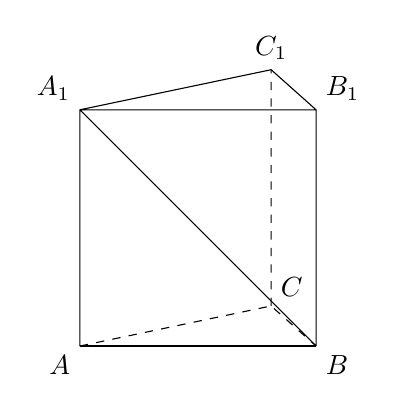
\begin{tikzpicture}[scale = 0.6]
        \draw (0,0) node [below left] {$A$} coordinate (A) -- (5,0) node [below right] {$B$} coordinate (B);
        \draw (3.2,0) + (45:1.2) node [above right] {$C$} coordinate (C);
        \draw [dashed] (A) -- (C) --(B);
        \draw (A) + (0,5) node [above left] {$A_1$} coordinate (A1);
        \draw (B) + (0,5) node [above right] {$B_1$} coordinate (B1);
        \draw (C) + (0,5) node [above] {$C_1$} coordinate (C1);
        \draw (A) -- (A1) -- (B1) -- (B) (A1) -- (C1) -- (B1) (A1) -- (B);
        \draw [dashed] (C) -- (C1);
    \end{tikzpicture}
\end{center}
\item 已知数列$\{a_n\}$, $\{b_n\}$满足$b_n=\ln a_n$, $n\in \mathbf{N}^*$, 其中$\{b_n\}$是等差数列, 且$a_3\cdot a_{1007}=\mathrm{e}^4$, 则$b_1+b_2+\cdots +b_{1009}=$\blank{50}.
\item 如图, 向量$\overrightarrow{OA}$与$\overrightarrow{OB}$的夹角为$120^\circ$, $|\overrightarrow{OA}|=2$, $|\overrightarrow{OB}|=1$, $P$是以$O$为圆心、$|\overrightarrow{OB}|$为半径的弧$\overset\frown{BC}$上的动点, 若$\overrightarrow{OP}=\lambda \overrightarrow{OA}+\mu \overrightarrow{OB}$, 则$\lambda \mu$的最大值是\blank{50}.
\begin{center}
    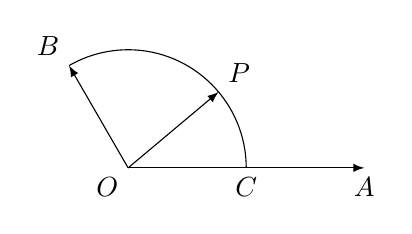
\begin{tikzpicture}[scale = 1.5, >=latex]
        \draw [->] (0,0) node [below left] {$O$} -- (2,0) node [below] {$A$};
        \draw [->] (0,0) --+ (120:1) node [above left] {$B$};
        \draw [->] (0,0) --+ (40:1) node [above right] {$P$};
        \draw (1,0) node [below] {$C$} arc (0:120:1);
    \end{tikzpicture}
\end{center}

% 赋能22

\item 设全集$U=\{ 1,2,3,4,5\}$, 若集合$A=\{3,4,5\}$, 则$\complement_U A=$\blank{50}.
\item 若$\sin\theta=\dfrac14$, 则$\cos(\dfrac{3 \pi}2+\theta)=$\blank{50}.
\item 方程$\log_2(2-x)+\log_2(3-x)=\log_2 12$的解$x=$\blank{50}.
\item $(\sqrt x-\dfrac1x)^9$的二项展开式中的常数项的值为\blank{50}.
\item 不等式$\dfrac1{|x-1|}\ge 1 $的解集为\blank{50}.
\item 函数$f(x)=\sqrt 3\sin x+2\cos^2\dfrac x2$的值域为\blank{50}.
\item 已知$\mathrm{i}$是虚数单位, $\overline z$是复数$z$的共轭复数, 若$\begin{vmatrix} z & 1+\mathrm{i}  \\ 1 & 2\mathrm{i} \end{vmatrix}=0$, 则$\overline z$在复平面内所对应的点所在的象限为第\blank{50}象限.
\item 若数列$\{a_n\}$的前$n$项和$S_n=-3n^2+2n+1 \ (n\in \mathbf{N}^*)$, 则$\displaystyle\lim_{n\to\infty}\dfrac{a_n}{3n}=$\blank{50}.
\item 若直线$l:x+y=5$与曲线$C:x^2+y^2=16$交于两点$A(x_1,y_1)$, $B(x_2,y_2)$, 则$x_1y_2+x_2y_1$的值为\blank{50}.
\item 设$a_1,a_2,a_3,a_4$是$1,2,3,4$的一个排列, 若至少有一个$i\ (i=1,2,3,4)$使得$a_i=i$成立, 则满足此条件的不同排列的个数为\blank{50}.

% 赋能23

\item 计算: $\displaystyle\lim_{n\to\infty}\dfrac{2n}{3n-1}=$\blank{50}.
\item 已知集合$A=\{x|0<x<3\}$, $B=\{x|x^2\ge 4\}$, 则$A\cap B=$\blank{50}.
\item 已知$\{a_n\}$为等差数列, $S_n$为其前$n$项和, 若$a_1+a_9=18$, $a_4=7 $, 则$S_{10}=$\blank{50}.
\item 已知函数$f(x)=\log_2(x+a)$的反函数为$y=f^{-1}(x)$, 且$f^{-1}(2)=1$, 则实数$a=$\blank{50}.
\item 已知角$\alpha$的终边与单位圆$x^2+y^2=1$交于点$P(\dfrac12,y_0)$, 则$\cos 2 \alpha$=\blank{50}.
\item 若存在$x\in [0,+\infty)$使$\begin{vmatrix}2^x & 2^x \\ m & x \end{vmatrix}<1$成立, 则实数$m$的取值范围是\blank{50}.
\item 函数$y=\sin 2x$的图像与$y=\cos x$的图像在区间$[0,2\pi]$上交点的个数是\blank{50}.
\item 若直线$ax-y+3=0$与圆$(x-1)^2+(y-2)^2=4$相交于$A$、$B$两点, 且$|AB|=2 \sqrt3$, 则$a$=\blank{50}.
\item 在$\triangle ABC$中, $\angle A=90^\circ $, $\triangle ABC$的面积为$1$. 若$\overrightarrow{BM}=\overrightarrow{MC}$, $\overrightarrow{BN}=4 \overrightarrow{NC}$, 则$\overrightarrow{AM}\cdot \overrightarrow{AN}$的最小值为\blank{50}.
\item 已知函数$f(x)=x|2x-a|-1$有三个零点, 则实数$a$的取值范围为\blank{50}.

% 赋能24

\item 设全集$U=\mathbf{Z}$, 集合$M=\{1,2\}$, $P=\{-2,-1,0,1,2\}$, 则$P\cap \complement_U M$=\blank{50}.
\item 已知复数$z=\dfrac{\mathrm{i}}{2+\mathrm{i}}$($\mathrm{i}$为虚数单位), 则$z\cdot \overline z$=\blank{50}.
\item 不等式$2^{x^2-4x-3}>(\dfrac12 )^{3(x-1)}$的解集为\blank{50}.
\item 函数$f(x)=\sqrt3\sin x\cos x+\cos^2x$的最大值为\blank{50}.
\item 在平面直角坐标系$xOy$中, 以直线$y=\pm 2x$为渐近线, 且经过椭圆$x^2+\dfrac{y^2}4=1$右顶点的双曲线的方程是\blank{50}.
\item 将圆锥的侧面展开后得到一个半径为$2$的半圆, 则此圆锥的体积为\blank{50}.
\item 设等差数列$\{a_n\}$的公差$d$不为$0$, $a_1=9d$. 若$a_k$是$a_1$与$a_{2k}$的等比中项, 则$k=$\blank{50}.
\item 已知$(1+2x)^6$展开式的二项式系数的最大值为$a$, 系数的最大值为$b$, 则$\dfrac ba=$\blank{50}.
\item 同时掷两枚质地均匀的骰子, 则两个点数之积不小于$4$的概率为\blank{50}.
\item 已知函数$f(x)=\begin{cases} \log_2 (x+a), & x\le 0, \\ x^2-3ax+a, & x>0 \end{cases}$有三个不同的零点, 则实数$a$的取值范围是\blank{50}.

% 赋能25

\item 在复平面内, 复数$\dfrac{5+4\mathrm{i}}{\mathrm{i}}$($\mathrm{i}$为虚数单位)对应的点的坐标为\blank{50}.
\item 函数$f(x)=\sqrt{1-\lg x}$的定义域为\blank{50}.
\item 二项式$(x-\dfrac1{2x})^4$的展开式中的常数项为\blank{50}.
\item 若$\begin{vmatrix} 4^x & 2 \\ 2^x & 1 \end{vmatrix}=0$, 则$x=$\blank{50}.
\item 已知圆$O:x^2+y^2=1$与圆$O'$关于直线$x+y=5$对称, 则圆$O'$的方程是\blank{50}.
\item 在坐标平面$xOy$内, $O$为坐标原点, 已知点$A(-\dfrac12,\dfrac{\sqrt3}2)$, 将$\overrightarrow{OA}$绕原点按顺时针方向旋转$\dfrac{\pi}2$, 得到$\overrightarrow{OA'}$, 则$\overrightarrow{OA'}$的坐标为\blank{50}.
\item 某船在海平面$A$处测得灯塔$B$在北偏东$30^\circ$方向, 与$A$相距$6.0$海里.船由$A$向正北方向航行$8.1$海里到达$C$处, 这时灯塔$B$与船相距\blank{50}海里(精确到$0.1$海里).
\item 若存在公差为$d$的等差数列$\{a_n\} \ (n\in \mathbf{N}^*)$满足$a_3a_4+1=0$, 则公差$d$的取值范围是\blank{50}.
\item 著名的斐波那契数列$\{a_n\}:1,1,2,3,5,8,\cdots$, 满足$a_1=a_2=1,a_{n+2}=a_{n+1}+a_n \ (n\in \mathbf{N}^*)$, 那么$1+a_3+a_5+a_7+a_9+\cdots+a_{2017}$是斐波那契数列中的第\blank{50}项.
\item 若不等式$(-1)^n\cdot a<3+\dfrac{(-1)^{n+1}}{n+1}$对任意正整数$n$恒成立, 则实数$a$的取值范围是\blank{50}.

%赋能26

\item 已知集合$A=\{1,2,m\}$, $B=\{3,4\}$.若$A\cap B=\{3\}$, 则实数$m=$\blank{50}.
\item 已知$\cos\theta=-\dfrac35$, 则$\sin(\theta+\dfrac{\pi}2)=$\blank{50}.
\item 若行列式$\begin{vmatrix} 2^{x-1} & 4  \\ 1 & 2 \end{vmatrix}$, 则$x=$\blank{50}.
\item 已知一个关于$x$, $y$的二元一次方程组的增广矩阵是$\begin{pmatrix} 1 & -1 & 2 \\ 0 & 1 & 2 \end{pmatrix}$, 则$x+y=$\blank{50}.
\item 在$(x-\dfrac2x)^6$的二项展开式中, 常数项的值为\blank{50}.
\item 若将一颗质地均匀的骰子(一种各面上分别标有1, 2, 3, 4, 5, 6六个点的正方体玩具), 先后抛掷2次, 则出现向上的点数之和为$4$的概率是\blank{50}.
\item 数列$\{a_n\}$的前$n$项和为$S_n$, 若点$(n,S_n) \ (n\in \mathbf{N}^*)$在函数$y=\log_2 (x+1)$的反函数的图像上, 则$a_n$=\blank{50}.
\item 在$\triangle ABC$中, 若$\sin A,\sin B,\sin C$成等比数列, 则角$B$的最大值为\blank{50}.
\item 抛物线$y^2=-8x$的焦点与双曲线$\dfrac{x^2}{a^2}-y^2=1$的左焦点重合, 则这条双曲线的两条渐近线的夹角为\blank{50}.
\item 已知函数$f(x)=\cos x(\sin x+\sqrt3\cos x)-\dfrac{\sqrt3}2$, $x\in \mathbf{R}$. 设$\alpha>0$, 若函数$g(x)=f(x+\alpha)$为 奇函数, 则$\alpha$的值为\blank{50}.

%赋能27

\item 不等式$\dfrac x{x+1}\le 0$的解集为\blank{50}.
\item 已知$\sin\alpha=\dfrac45$, 则$\cos(\alpha+\dfrac{\pi}2)=$\blank{50}.
\item $\displaystyle\lim_{n\to\infty}\dfrac{3^n-1}{3^{n+1}+1}=$\blank{50}.
\item 已知球的表面积为$16\pi$, 则该球的体积为\blank{50}.
\item 已知函数$f(x)=1+\log_a x$, $y=f^{-1}(x)$是函数$y=f(x)$的反函数, 若$y=f^{-1}(x)$的图像过点$(2,4)$, 则$a$的值为\blank{50}.
\item 若数列$\{a_n\}$为等比数列, 且$a_5=3$, 则$\begin{vmatrix} a_2 & -a_7 \\ a_3 & a_8 \end{vmatrix}=$\blank{50}.
\item 在$\triangle ABC$中, 角$A$、$B$、$C$所对的边分别为$a$、$b$、$c$, 若$(a+b+c)(a-b+c)=ac$, 则$B=$\blank{50}.
\item 若$(2x+\dfrac 1x)^n$的二项展开式中的所有二项式系数之和等于$256$, 则该展开式中常数项的值为\blank{50}.
\item 已知函数$f(x)$是定义在$\mathbf{R}$上且周期为$4$的偶函数. 当$x\in [2,4]$时, $f(x)=\left|\log_4(x-\dfrac32)\right|$, 则$f(\dfrac12)$的值为\blank{50}.
\item 已知数列$\{a_n\}$的前$n$项和为$S_n$, 且$a_1=1$, $2S_n=a_na_{n+1}$($n\in \mathbf{N}^*$), 若$b_n=(-1)^n\dfrac{2n+1}{{a_n}{a_{n+1}}}$, 则数列$\{b_n\}$的前$n$项和$T_n=$\blank{50}.

%赋能28

\item 设全集$U=\{1,2,3,4\}$, 集合$A=\{x|x^2-5x+4<0,x\in \mathbf{Z}\}$, 则$\complement_U A$=\blank{50}.
\item 参数方程为$\begin{cases} x=t^2, \\ y=2t, \end{cases}$ ($t$为参数)的曲线的焦点坐标为\blank{50}.
\item 已知复数$z$满足$|z|=1$, 则$|z-2|$的取值范围是\blank{50}.
\item 设数列$\{a_n\}$的前$n$项和为$S_n$, 若$S_n=1-\dfrac23{a_n} \ (n\in \mathbf{N}^*)$, 则$\displaystyle\lim_{n\to\infty}S_n$=\blank{50}.
\item 若$(x+\dfrac1{2x})^n \ (n\ge 4, \ n\in \mathbf{N}^*)$的二项展开式中前三项的系数依次成等差数列, 则$n=$\blank{50}.
\item 把$1,2,3,4,5,6,7,8,9,10$分别写在$10$张形状大小一样的卡片上, 随机抽取一张卡片, 则抽到写着偶数或大于$6$的数的卡片的概率为\blank{50}(结果用最简分数表示).
\item 若行列式$\begin{vmatrix} 1 & 2 & 4 \\ \cos \dfrac x2 & \sin \dfrac x2 & 0 \\ \sin \dfrac x2 & \cos \dfrac x2 & 8 \end{vmatrix}$中元素$4$的代数余子式的值为$\dfrac12$, 则实数$x$的取值集合为\blank{50}.
\item 满足约束条件$|x|+2|y|\le 2$的目标函数$z=y-x$的最小值是\blank{50}.
\item 已知函数$f(x)=\begin{cases} \log_2 x, & 0<x<2, \\ (\dfrac23)^x+\dfrac59, & x\ge 2. \end{cases}$ 若函数$g(x)=f(x)-k$有两个不同的零点, 则实数$k$的取值范围是\blank{50}.
\item 某部门有$8$位员工, 其中$6$位员工的月工资分别为$8200$, $8300$, $8500$, $9100$, $9500$, $9600$(单位: 元), 另两位员工的月工资数据不清楚, 但两人的月工资和为$17000$元, 则这$8$位员工月工资的中位数可能的最大值为\blank{50}元.

% 赋能29

\item 计算: $\displaystyle\lim_{n\to\infty}(1+\dfrac1n)^3=$\blank{50}.
\item 函数$y=\log_2(1-\dfrac1x)$的定义域为\blank{50}.
\item 若$\dfrac{\pi}2<\alpha<\pi$, $\sin\alpha=\dfrac35$, 则$\tan\dfrac{\alpha}2=$\blank{50}.
\item 若复数$z=(1+\mathrm{i})\cdot \mathrm{i}^2$($\mathrm{i}$表示虚数单位), 则$\overline z=$\blank{50}.
\item 曲线$C$: $\begin{cases} x=\sec\theta, \\ y=\tan\theta, \end{cases}$($\theta$为参数)的两个顶点之间的距离为\blank{50}.
\item 若从一副$52$张的扑克牌中随机抽取$2$张, 则在放回抽取的情形下, 两张牌都是K的概率为\blank{50}(结果用最简分数表示).
\item 若关于$x$的方程$\sin x+\cos x-m=0$在区间$[0,\dfrac{\pi}2]$上有解, 则实数$m$的取值范围是\blank{50}.
\item 若一个圆锥的母线与底面所成的角为$\dfrac{\pi}6$,体积为$125\pi$,则此圆锥的高为\blank{50}.
\item 若函数$f(x)=\log_2^2x-\log_2 x+1 \ (x\ge 2)$的反函数为$f^{-1}(x)$, 则$f^{-1}(3)$=\blank{50}.
\item 若三棱锥$S-ABC$的所有的顶点都在球$O$的球面上, $SA\perp$平面$ABC$, $SA=AB=2$, $AC=4$, $\angle BAC=\dfrac{\pi}3$, 则球$O$的表面积为\blank{50}.

% 赋能30

\item 方程$\log_3(2x+1)=2$的解是\blank{50}.
\item 已知集合$M=\{x||x+1|\le 1\},N=\{-1,0,1\},$则$M\cap N=$\blank{50}.
\item 若复数$z_1=a+2\mathrm{i}$, $z_2=2+\mathrm{i}$($\mathrm{i}$是虚数单位), 且$z_1z_2$为纯虚数, 则实数$a$=\blank{50}.
\item 直线$\begin{cases} x=-2-\sqrt2 t,  \\y=3+\sqrt2 t, \end{cases}$($t$为参数)对应的普通方程是\blank{50}.
\item 若$(x+2)^n=x^n+ax^{n-1}+\cdots+bx+c \ (n\in \mathbf{N}^*, \ n\ge 3)$, 且$b=4c$, 则$a$的值为\blank{50}.
\item 某空间几何体的三视图如图所示, 则该几何体的侧面积是\blank{50}.
\begin{center}
    \begin{tikzpicture}[>=latex]
        \draw (0,0) circle (1);
        \draw (-1,-1.1) -- (-1,-1.3) (1,-1.1) -- (1,-1.3);
        \draw [->] (-0.2,-1.2) -- (-1,-1.2);
        \draw [->] (0.2,-1.2) -- (1,-1.2);
        \draw (0,-1.2) node {$4$};
        \draw (0,-1.6) node {俯视图};
        \draw (-1,2) -- (1,2) -- (0,5) -- cycle;
        \draw (0,1.4) node {主视图};
        \draw (-1,1.9) -- (-1,1.7) (1,1.9) -- (1,1.7);
        \draw [->] (-0.2,1.8) -- (-1,1.8);
        \draw [->] (0.2,1.8) -- (1,1.8);
        \draw (0,1.8) node {$4$};
        \draw (1.1,2) -- (1.3,2) (1.1,5) -- (1.3,5);
        \draw [->] (1.2,3.2) -- (1.2,2);
        \draw [->] (1.2,3.8) -- (1.2,5);
        \draw (1.2,3.5) node {$6$};
        \draw (2,2) -- (4,2) -- (3,5) -- cycle;
        \draw (3,1.4) node {左视图};
        \draw (2,1.9) -- (2,1.7) (4,1.9) -- (4,1.7);
        \draw [->] (2.8,1.8) -- (2,1.8);
        \draw [->] (3.2,1.8) -- (4,1.8);
        \draw (3,1.8) node {$4$};
        \draw (4.1,2) -- (4.3,2) (4.1,5) -- (4.3,5);
        \draw [->] (4.2,3.2) -- (4.2,2);
        \draw [->] (4.2,3.8) -- (4.2,5);
        \draw (4.2,3.5) node {$6$};
    \end{tikzpicture}
\end{center}
\item 若函数$f(x)=2^x(x+a)-1$在区间$[0,1]$上有零点, 则实数$a$的取值范围是\blank{50}.
\item 在约束条件$|x+1|+|y-2|\le 3$下, 目标函数$z=x+2y$的最大值为\blank{50}.
\item 某学生在上学的路上要经过$2$个路口, 假设在各路口是否遇到红灯是相互独立的, 遇到红灯的概率都是$\dfrac13$, 则这名学生在上学的路上到第二个路口时第一次遇到红灯的概率是\blank{50}.
\item 已知椭圆$x^2+\dfrac{y^2}{b^2}=1\ (0<b<1)$, 其左、右焦点分别为$F_1$, $F_2$, $|F_1F_2|=2c$. 若此椭圆上存在点$P$, 使$P$到直线$x=\dfrac1c$的距离是$|PF_1|$与$|PF_2|$的等差中项, 则$b$的最大值为\blank{50}.

% 赋能31

\item 函数$y=1-2\sin^2(2x)$的最小正周期是\blank{50}.
\item 若全集$U=\mathbf{R}$, 集合$A=\{x|x\ge 1\}\cup\{x|x<0\}$, 则$\complement_U A=$\blank{50}.
\item 若复数$z$满足$z+\mathrm{i}=\dfrac{2+\mathrm{i}}{\mathrm{i}}$($\mathrm{i}$为虚数单位), 则$|z|=$\blank{50}.
\item 设$m$为常数, 若点$F(0,5)$是双曲线$\dfrac{y^2}m-\dfrac{x^2}9=1$的一个焦点, 则$m=$\blank{50}.
\item 已知正四棱锥的底面边长是$2$, 侧棱长是$\sqrt3$, 则该正四棱锥的体积为\blank{50}.
\item 若实数$x,y$满足$\begin{cases} x-y+1 \le 0, \\ x+y-3 \ge 0, \\ y\le 4,\end{cases}$ 则目标函数$z=2x-y$的最大值为\blank{50}.
\item 若$(\sqrt x-\dfrac1x)^n$的二项展开式中各项的二项式系数的和是$64$, 则展开式中的常数项的值为\blank{50}.
\item 数列$\{a_n\}$是等比数列, 前n项和为$S_n$, 若$a_1+a_2=2$, $a_2+a_3=-1$, 则$\displaystyle\lim_{n\to\infty}{S_n}=$\blank{50}.
\item 若函数$f(x)=4^x+2^{x+1}$的图像与函数$y=g(x)$的图像关于直线$y=x$对称, 则$g(3)=$\blank{50}.
\item 甲与其四位朋友各有一辆私家车, 甲的车牌尾数是$0$, 其四位朋友的车牌尾数分别是$0$, $2$, $1$, $5$, 为遵守当地4月1日至5日$5$天的限行规定(奇数日车牌尾数为奇数的车通行, 偶数日车牌尾数为偶数的车通行), 五人商议拼车出行, 每天任选一辆符合规定的车, 但甲的车最多只能用一天, 则不同的用车方案总数为\blank{50}.

% 赋能32

\item 集合$A=\{1,2,3,4\}$, $B=\{x|(x-1)(x-5)<0\}$, 则$A\cap B=$\blank{50}.
\item 复数$z=\dfrac{2-\mathrm{i}}{1+\mathrm{i}}$所对应的点在复平面内位于第\blank{50}象限.
\item 已知首项为$1$公差为$2$的等差数列$\{a_n\}$, 其前$n$项和为$S_n$, 则$\displaystyle\lim_{n\to\infty}\dfrac{a_n^2}{S_n}=$\blank{50}.
\item 若方程组$\begin{cases} ax+2y=3, \\ 2x+ay=2 \end{cases}$ 无解, 则实数$a=$\blank{50}.
\item 若$(x+a)^7$的二项展开式中, 含$x^6$项的系数为$7$, 则实数$a=$\blank{50}.
\item 已知双曲线$x^2-\dfrac{y^2}{a^2}=1 \ (a>0)$,它的渐近线方程是$y=\pm 2x$,则$a$的值为\blank{50}.
\item 在$\triangle ABC$中, 三边长分别为$a=2$, $b=3$, $c=4$, 则$\dfrac{\sin 2A}{\sin B}=$\blank{50}.
\item 在平面直角坐标系中, 已知点$P(-2,2)$, 对于任意不全为零的实数$a$、$b$, 直线$l:a(x-1)+b(y+2)=0$, 若点$P$到直线$l$的距离为$d$, 则$d$的取值范围是\blank{50}.
\item 函数$f(x)=\begin{cases} |x|, & x\le 1,  \\ (x-2)^2, & x>1, \end{cases}$ 如果方程$f(x)=b$有四个不同的实数解$x_1$、$x_2$、$x_3$、$x_4$, 则${x_1}+{x_2}+{x_3}+{x_4}=$\blank{50}.
\item 三条侧棱两两垂直的正三棱锥, 其俯视图如图所示, 主视图的边界是底边长为$2$的等腰三角形, 则主视图的面积等于\blank{50}.
\begin{center}
    \begin{tikzpicture}[scale = 1.5, >=latex]
        \draw (0,0) -- (2,0) -- (1,{sqrt(3)}) coordinate (T) -- cycle;
        \draw (0,0) -- (1,{sqrt(3)/3}) -- (2,0) (1,{sqrt(3)/3}) -- (1,{sqrt(3)});
        \draw (0,-0.1) -- (0,-0.3) (2,-0.1) -- (2,-0.3);
        \draw (1,-0.2) node {$2$};
        \draw [->] (0.8,-0.2) -- (0,-0.2);
        \draw [->] (1.2,-0.2) -- (2,-0.2);
        \draw (1,-0.5) node {俯视图};
        \draw (2,0) ++ (30:0.1) --++ (30:0.2) (T) ++ (30:0.1) --++ (30:0.2);
        \draw [->] ($(2,0)!0.4!(T)$) ++ (30:0.2) --+ (-60:0.8);
        \draw [->] ($(2,0)!0.6!(T)$) ++ (30:0.2) --+ (120:0.8);
        \draw ($(2,0)!0.5!(T)$) ++ (30:0.2) node {$2$};
        \draw (0,0) ++ (150:0.1) --++ (150:0.2) (T) ++ (150:0.1) --++ (150:0.2);
        \draw [->] ($(0,0)!0.4!(T)$) ++ (150:0.2) --+ (240:0.8);
        \draw [->] ($(0,0)!0.6!(T)$) ++ (150:0.2) --+ (60:0.8);
        \draw ($(0,0)!0.5!(T)$) ++ (150:0.2) node {$2$};
    \end{tikzpicture}
\end{center}

% 赋能33

\item 函数$y=\sqrt{2x-x^2}$的定义域是\blank{50}.
\item 若关于$x,y$的方程组$\begin{cases} ax+y-1=0,  \\ 4x+ay-2=0  \end{cases}$有无数多组解, 则实数$a=$\blank{50}.
\item 若``$x^2-2x-3>0$''是``$x<a$''的必要不充分条件, 则$a$的最大值为\blank{50}.
\item 已知复数$z_1=3+4\mathrm{i}$, $z_2=t+\mathrm{i}$(其中$\mathrm{i}$为虚数单位), 且$z_1\cdot \overline{z_2}$是实数, 则实数$t$等于\blank{50}.
\item 若函数$f(x)=\begin{cases} -x+3a, & x<0,  \\ a^x+1, & x\ge 0 \end{cases}$($a>0$, 且$a\ne 1$)是$\mathbf{R}$上的减函数, 则$a$的取值范围是\blank{50}.
\item 设变量$x,y$满足约束条件$\begin{cases} x+y\ge 2, \\ x-y\le 1, \\ y\le 2,\end{cases}$ 则目标函数$z=-2x+y$的最小值为\blank{50}.
\item 已知圆$C:(x-4)^2+(y-3)^2=4$和两点$A(-m,0)$, $B(m,0)$($m>0$), 若圆$C$上至少存在一点$P$, 使得$\angle APB=90^\circ $, 则$m$的取值范围是\blank{50}.
\item 已知向量$\overrightarrow a=(\cos(\dfrac{\pi}3+\alpha),1)$, $\overrightarrow b=(1,4)$, 如果$\overrightarrow a \parallel \overrightarrow b$, 那么$\cos(\dfrac{\pi}3-2\alpha)$的值为\blank{50}.
\item 若从正八边形的$8$个顶点中随机选取$3$个顶点, 则以它们作为顶点的三角形是直角三角形的概率是\blank{50}.
\item 若将函数$f(x)=|\sin(\omega x-\dfrac{\pi}8)| \ (\omega >0)$的图像向左平移$\dfrac{\pi}{12}$个单位后, 所得图像对应的函数为偶函数, 则$\omega$的最小值是\blank{50}.

% 赋能34

\item 已知集合$A=\{x|\ln x>0 \}$, $B=\{x|2^x<3\}$, 则\blank{50}.
\item 若实数$x$, $y$满足约束条件$\begin{cases} x\ge 0, \\  y\le x, \\  2x+y-9 \le 0, \end{cases}$ 则$z=x+3y$的最大值等于\blank{50}.
\item 已知$(x-\dfrac ax)^7$展开式中$x^3$的系数为$84$, 则正实数$a$的值为\blank{50}.
\item 盒中装有形状、大小完全相同的$5$个球, 其中红色球$3$个, 黄色球$2$个. 若从中随机取出$2$个球, 则所取出的$2$个球颜色不同的概率为\blank{50}.
\item 设$f(x)$为$\mathbf{R}$上的奇函数. 当$x\ge 0$时, $f(x)=2^x+2x+b$($b$为常数), 则$f(-1)$的值为\blank{50}.
\item 设$P,Q$分别为直线$\begin{cases}  x=t, \\  y=6-2t, \end{cases}$($t$为参数)和曲线$C:\begin{cases} x=1+\sqrt5\cos\theta, \\ y=-2+\sqrt5\sin\theta,\end{cases}$($\theta$为参数)的点, 则$|PQ|$的最小值为\blank{50}.
\item 各项均不为零的数列$\{a_n\}$的前$n$项和为$S_n$.  对任意$n\in \mathbf{N}^*$, $\overrightarrow{m_n}=(a_{n+1}-a_n,2a_{n+1})$
都是直线$y=kx$的法向量. 若$\displaystyle\lim_{n\to\infty}S_n$存在, 则实数$k$的取值范围是\blank{50}.
\item 已知正四棱锥$P-ABCD$的棱长都相等, 侧棱$PB$、$PD$的中点分别为$M$、$N$, 则截面$AMN$与底面$ABCD$所成的二面角的余弦值是\blank{50}.
\item 设$a>0$, 若对于任意的$x>0$, 都有$\dfrac1a-\dfrac1x\le 2x$, 则$a$的取值范围是\blank{50}.
\item 若适合不等式$|x^2-4x+k|+|x-3|\le 5$的$x$的最大值为$3$, 则实数$k$的值为\blank{50}.

% 赋能35

\item 已知集合$A=\{x|\dfrac{x-2}{x+1}\ge 0\}$, 集合$B=\{y|0 \le y<4\}$, 则$A\cap B$=\blank{50}.
\item 若直线$l$的参数方程为$\begin{cases} x=4-4t,  \\ y=-2+3t,\end{cases} \  t\in \mathbf{R}$, 则直线$l$在$y$轴上的截距是\blank{50}.
\item 已知圆锥的母线长为$4$, 母线与旋转轴的夹角为$30^\circ$, 则该圆锥的侧面积为\blank{50}.
\item 抛物线$y=\dfrac14{x^2}$的焦点到准线的距离为\blank{50}.
\item 已知关于$x,y$的二元一次方程组的增广矩阵为$\begin{pmatrix} 2 & 1 & 5  \\ 1 & -2 & 0 \end{pmatrix}$, 则$3x-y$=\blank{50}.
\item 若三个数$a_1,a_2,a_3$的方差为$1$, 则$3a_1+2,3a_2+2,3a_3+2$的方差为\blank{50}.
\item 已知射手甲击中A目标的概率为$0.9$, 射手乙击中A目标的概率为$0.8$, 若甲、乙两人各向A目标射击一次, 则射手甲或射手乙击中A目标的概率是\blank{50}.
\item 函数$y=\sin (\dfrac{\pi}6-x), \ x\in [0,\dfrac32\pi]$的单调递减区间是\blank{50}.
\item 已知等差数列$\{a_n\}$的公差为$2$, 前$n$项和为$S_n$, 则$\displaystyle\lim_{n\to\infty}\dfrac{S_n}{{a_n}{a_{n+1}}}$=\blank{50}.
\item 已知定义在$\mathbf{R}$上的函数$f(x)$满足: \textcircled{1} $f(x)+f(2-x)=0$; \textcircled{2} $f(x)-f(-2-x)=0$; \textcircled{3} 在$[-1,1]$上的表达式为$f(x)=\begin{cases} \sqrt{1-x^2}, & x\in [-1,0], \\ 1-x, & x\in (0,1] \end{cases}$, 则函数$f(x)$与函数$g(x)=\begin{cases} 2^x, & x\le 0, \\ \log_{\frac12} x,& x>0 \end{cases}$的图像在区间$[-3,3]$上的交点的个数为\blank{50}.

% 赋能36

\item 函数$y=2\sin^2(2x)-1$的最小正周期是\blank{50}.
\item 设$\mathrm{i}$为虚数单位, 复数$z=\dfrac{1-2 \mathrm{i}}{2+\mathrm{i}}$, 则$|z|=$\blank{50}.
\item 设$f^{-1}(x)$为$f(x)=\dfrac{2x}{x+1}$的反函数, 则$f^{-1}(1)=$\blank{50}.
\item $\displaystyle\lim_{n\to\infty}\dfrac{2^{n+1}+3^{n+1}}{2^n+3^n}=$\blank{50}.
\item 若圆锥的侧面积是底面积的$2$倍, 则其母线与轴所成角的大小是\blank{50}.
\item 设等差数列$\{a_n\}$的前$n$项和为$S_n$, 若$\dfrac{a_5}{a_3}=\dfrac53$, 则$\dfrac{S_5}{S_3}=$\blank{50}.
\item 直线$\begin{cases} x=2+t, \\ y=4-t,\end{cases}$($t$为参数)与曲线$\begin{cases} x=3+\sqrt2\cos\theta, \\ y=5+\sqrt2\sin\theta \end{cases}$($\theta$为参数)的公共点的个数是\blank{50}.
\item 已知双曲线$C_1$与双曲线$C_2$的焦点重合,$C_1$的方程为$\dfrac{x^2}3-{y^2}=1$, 若$C_2$的一条渐近线的倾斜角是$C_1$的一条渐近线的倾斜角的$2$倍, 则$C_2$的方程为\blank{50}.
\item 若$f(x)={x^{\frac13}}-{x^{-\frac12}}$, 则满足$f(x)>0$的$x$的取值范围是\blank{50}.
\item 某企业有甲、乙两个研发小组, 他们研发新产品成功的概率分别为$\dfrac23$和$\dfrac35$. 现安排甲组研发新产品A, 乙组研发新产品B, 设甲、乙两组的研发相互独立 , 则至少有一种新产品研发成功的概率为\blank{50}.

% 赋能37

\item 已知集合$A=\{x|x>-1, \ x\in \mathbf{R}\}$, 集合$B=\{x|x<2, \ x\in \mathbf{R}\}$, 则$A\cap B=$\blank{50}.
\item 已知复数$z$满足$(2-3\mathrm{i})z=3+2\mathrm{i}$($i$为虚数单位), 则$|z|=$\blank{50}.
\item 函数$f(x)=\begin{vmatrix} \sin x & 2\cos x \\ 2\cos x & \sin x\end{vmatrix}$的最小正周期是\blank{50}.
\item 已知双曲线$\dfrac{x^2}{a^2}-\dfrac{y^2}{(a+3)^2}=1 \ (a>0)$的一条渐近线方程为$y=\pm 2x$, 则$a=$\blank{50}.
\item 若圆柱的侧面展开图是边长为$4\text{cm}$的正方形, 则圆柱的体积为\blank{50}$\text{cm}^3$(结果精确到$0.1\text{cm}^3$).
\item 已知$x,y$满足$\begin{cases} x-y\le 0,\\ x+y\le 2, \\ x+2 \ge 0,\end{cases}$ 则$z=2x+y$的最大值是\blank{50}.
\item 直线$\begin{cases} x=t-1, \\ y=2-t,\end{cases}$($t$为参数)与曲线$\begin{cases} x=3\cos\theta, \\ y=2\sin\theta,\end{cases}$($\theta$为参数)的交点个数是\blank{50}.
\item 已知函数$f(x)=\begin{cases}2^x, & x\le 0, \\ \log_2 x, & 0<x\le 1\end{cases}$的反函数是$f^{-1}(x)$, 则$f^{-1}(\dfrac12)=$\blank{50}.
\item 设多项式$1+x+(1+x)^2+(1+x)^3+\cdots+(1+x)^n\ (x\ne 0, \ n\in \mathbf{N}^*)$的展开式中$x$项的系数为$T_n$, 则$\displaystyle\lim_{n\to \infty}\dfrac{T_n}{n^2}=$\blank{50}.
\item 生产零件需要经过两道工序, 在第一、第二道工序中产生废品的概率分别为$0.01$和$p$, 每道工序产生废品相互独立. 若经过两道工序后得到的零件不是废品的概率是$0.9603$, 则$p=$\blank{50}.

% 赋能38

\item 行列式$\begin{vmatrix} 1 & 2 & 3 \\ 4 & 5 & 6  \\ 7 & 8 & 9 \end{vmatrix}$中, 元素$5$的代数余子式的值为\blank{50}.
\item 设实数$\omega>0$, 若函数$f(x)=\cos(\omega x)+\sin(\omega x)$的最小正周期为$\pi$, 则$\omega=$\blank{50}.
\item 已知圆锥的底面半径和高均为$1$, 则该圆锥的侧面积为\blank{50}.
\item 设向量$\overrightarrow{a}=(2,3)$, 向量$\overrightarrow{b}=(6,t)$. 若$\overrightarrow{a}$与$\overrightarrow{b}$的夹角为钝角, 则实数$t$的取值范围为\blank{50}.
\item 集合$A=\{1,3,a^2\}$, 集合$B=\{a+1,a+2\}$. 若$B\cup A=A$, 则实数$a=$\blank{50}.
\item 设$z_1,z_2$是方程$z^2+2z+3=0$的两根, 则$|z_1-z_2|=$\blank{50}.
\item 设$f(x)$是定义在$\mathbf{R}$上的奇函数, 当$x>0$时,$f(x)=2^x-3$. 则不等式$f(x)<-5$的解为\blank{50}.
\item 若变量$x,y$满足约束条件$\begin{cases} x+y\le 12, \\ 2x-y\ge 0,  \\ x-2y\le 0, \end{cases}$ 则$z=y-x$的最小值为\blank{50}.
\item 小明和小红各自掷一颗均匀的正方体骰子, 两人相互独立地进行. 则小明掷出的点数不大于$2$或小红掷出的点数不小于$3$的概率为\blank{50}.
\item 设$A$是椭圆$\dfrac{x^2}{a^2}+\dfrac{y^2}{a^2-4}=1 \ (a>0)$上的动点, 点$F$的坐标为$(-2,0)$, 若满足$|AF|=10$的点$A$有且仅有两个, 则实数$a$的取值范围为\blank{50}.

% 赋能39

\item 设全集$U=\mathbf{R}$, 若集合$A=\{2\}$,$B=\{x|-1<x<2\}$, 则$A\cap (\complement_UB)=$\blank{50}.
\item 设抛物线的焦点坐标为$(1,0)$, 则此抛物线的标准方程为\blank{50}.
\item 某次体检, $8$位同学的身高(单位: 米)分别为. $1.68$, $1.71$, $1.73$, $1.63$, $1.81$, $1.74$, $1.66$, $1.78$, 则这组数据的中位数是\blank{50}(米).
\item 函数$f(x)=2\sin 4x \cos 4x$的最小正周期为\blank{50}.
\item 已知球的俯视图面积为$\pi$, 则该球的表面积为\blank{50}.
\item 若线性方程组的增广矩阵为$\begin{pmatrix} 1 & 2 & c_1 \\ 2 & 0 & c_2\end{pmatrix}$、解为$\begin{cases}x=1, \\ y=3,\end{cases}$ 则$c_1+c_2=$\blank{50}.
\item 在报名的$8$名男生和$5$名女生中, 选取$6$人参加志愿者活动, 要求男、女生都有, 则不同的选取方式的种数为\blank{50}(结果用数值表示).
\item 设无穷等比数列$\{a_n\}$的公比为$q$, 若$a_2=\displaystyle\lim_{n\to\infty}(a_4+a_5+\cdots+a_n)$, 则$q=$\blank{50}.
\item 若事件$A$、$B$满足$P(A)=\dfrac12$, $P(B)=\dfrac45$, $P(AB)=\dfrac25$, 则$P(\overline A B)-P(A\overline B)=$\blank{50}.
\item 设奇函数$f(x)$的定义域为$\mathbf{R}$, 当$x>0$时,$f(x)=x+\dfrac{m^2}x-1$(这里$m$为正常数). 若$f(x)\le m-2$对一切$x\le 0$成立, 则$m$的取值范围为\blank{50}.

% 赋能40

\item 已知集合$U=\{-1,0,1,2,-3\}$, $A=\{-1,0,2\}$, 则$\complement_U A=$\blank{50}.
\item 已知一个关于$x,y$的二元一次方程组的增广矩阵是$\begin{pmatrix} 1 & -1 & 1  \\ 0 & 1 & 2 \end{pmatrix}$, 则$x+y=$\blank{50}.
\item $\mathrm{i}$是虚数单位, 若复数$(1-2\mathrm{i})(a+\mathrm{i})$是纯虚数, 则实数$a$的值为\blank{50}.
\item 若$\begin{vmatrix} \log_2 x & -1  \\ -4 & 2  \end{vmatrix}=0$, 则$x=$\blank{50}.
\item 我国古代数学名著《九章算术》有``米谷粒分''题: 粮仓开仓收粮, 有人送来米$1534$石, 验得米内夹谷, 抽样取米一把, 数得$254$粒内夹谷$28$粒, 则这批米内夹谷约为\blank{50}石(精确到小数点后一位数字).
\item 已知圆锥的母线长为$5$, 侧面积为$15\pi$, 则此圆锥的体积为\blank{50}(结果保留$\pi$).
\item 若二项式$(2x+\dfrac ax)^7$的展开式中一次项的系数是$-70$, 则$\displaystyle\lim_{n\to\infty}(a+a^2+a^3+\cdots+a^n)=$\blank{50}.
\item 已知椭圆$\dfrac{x^2}{a^2}+y^2=1 \ (a>0)$的焦点$F_1$、$F_2$, 抛物线${y^2}=2x$的焦点为$F$, 若$\overrightarrow{F_1F}=3 \overrightarrow{FF_2}$, 则$a=$\blank{50}.
\item 设$f(x)$是定义在$\mathbf{R}$上以$2$为周期的偶函数, 当$x\in [0,1]$时, $f(x)=\log_2(x+1)$, 则函数$f(x)$在$[1,2]$上的解析式是\blank{50}.
\item 已知$x,y\in \mathbf{R}$, 且满足$\begin{cases} \sqrt3x+y\le 4 \sqrt3, \\  \sqrt3x-y\ge 0,\\ y\ge 0. \end{cases}$ 若存在$\theta \in \mathbf{R}$使得$x\cos \theta +y\sin \theta +1=0$成立, 则点$P(x,y)$构成的区域面积为\blank{50}.

% 赋能41

\item 集合$A=\{x|\dfrac x{x-2}<0\}$,$B=\{x|x\in \mathbf{Z}\}$, 则$A\cap B$等于\blank{50}.
\item 已知半径为$2R$和$R$的两个球, 则大球和小球的体积比为\blank{50}.
\item 抛物线$y=x^2$的焦点坐标是\blank{50}.
\item 已知实数$x,y$满足$\begin{cases} x-2\le 0, \\ y-1\le 0, \\ x+y\ge 2,\end{cases}$ 则目标函数$u=x+2y$的最大值是\blank{50}.
\item 已知在$\triangle ABC$中, $a$, $b$, $c$分别为$\angle A$, $\angle B$, $\angle C$所对的边. 若$b^2+c^2-a^2=\sqrt{2}bc$, 则$\angle A=$\blank{50}.
\item 三阶行列式$\begin{vmatrix}-5 & 6 & 7  \\ 4 & 2^x & 1  \\ 0 & 3 & 1  \end{vmatrix}$中元素$-5$的代数余子式为$f(x)$, 则方程$f(x)=0$的解为\blank{50}.
\item 设$z$是复数,$a(z)$表示满足$z^n=1$时的最小正整数$n$, $\mathrm{i}$是虚数单位, 则$a(\dfrac{1+\mathrm{i}}{1-\mathrm{i}})=$\blank{50}.
\item 无穷等比数列$\{a_n\}$的通项公式$a_n=(\sin x)^n$, 前$n$项的和为$S_n$, 若$\displaystyle\lim_{n\to\infty}S_n=1$, $x\in (0,\pi)$, 则$x=$\blank{50}.
\item 给出下列函数: \textcircled{1} $y=x+\dfrac1x$; \textcircled{2} $y={x^2}+x$; \textcircled{3} $y={2^{|x|}}$; \textcircled{4} $y={x^{\dfrac23}}$; \textcircled{5} $y=\tan x$; \textcircled{6} $y=\sin(\arccos x)$; \textcircled{7} $y=\lg(x+\sqrt{{x^2}+4})-\lg 2$. 从这$7$个函数中任取两个函数, 则其中一个是奇函数另一个是偶函数的概率是\blank{50}.
\item 代数式$(x^2+2)(\dfrac1{x^2}-1)^5$的展开式的常数项是\blank{50}(用数字作答).

% 赋能42

\item 已知全集$U=\mathbf{R}$, 集合$A=\{x|x^2-2x-3>0\}$, 则$\complement_U A=$\blank{50}.
\item 在$(x+\dfrac1x)^6$的二项展开式中, 常数项是\blank{50}.
\item 函数$f(x)=\lg (3^x-2^x)$的定义域为\blank{50}.
\item 已知抛物线$x^2=ay$的准线方程是$y=-\dfrac14$, 则$a=$\blank{50}.
\item 若一个球的体积为$\dfrac{32\pi}3$, 则该球的表面积为\blank{50}.
\item 已知实数$x,y$满足$\begin{cases} x\ge 0, \\ y\ge 0, \\ x+y\le 1, \end{cases}$ 则目标函数$z=x-y$的最小值为\blank{50}.
\item 函数$f(x)=\begin{vmatrix} (\sin x+\cos x)^2 & -1 \\ 1 & 1 \end{vmatrix}$的最小正周期是\blank{50}.
\item 若一圆锥的底面半径为$3$, 体积是$12\pi$, 则该圆锥的侧面积等于\blank{50}.
\item 将两颗质地均匀的骰子抛掷一次, 记第一颗骰子出现的点数是$m$, 记第二颗骰子出现的点数是$n$, 向量$\overrightarrow a=(m-2,2-n)$, 向量$\overrightarrow b=(1,1)$, 则向量$\overrightarrow a\perp \overrightarrow b$的概率是\blank{50}.
\item 已知直线$l_1:mx-y=0$, $l_2:x+my-m-2=0$. 当$m$在实数范围内变化时, $l_1$与$l_2$的交点$P$恒在一个定圆上, 则定圆方程是\blank{50}.

% 赋能43

\item 已知$A=(-\infty,a]$, $B=[1,2]$, 且$A\cap B\ne \varnothing$, 则实数$a$的范围是\blank{50}.
\item 直线$ax+(a-1)y+1=0$与直线$4x+ay-2=0$互相平行, 则实数$a=$\blank{50}.
\item 已知$\alpha \in (0,\pi)$, $\cos\alpha =-\dfrac35$, 则$\tan(\alpha+\dfrac{\pi}4)=$\blank{50}.
\item 长方体的对角线与过同一个顶点的三个表面所成的角分别为$\alpha$, $\beta$, $\gamma$, 则$\cos^2\alpha+\cos^2\beta+\cos^2\gamma =$\blank{50}.
\item 已知函数$f(x)=\begin{cases} -x^2, & x\ge 0,  \\2^{-x}-1, & x<0, \end{cases}$ 则$f^{-1}[f^{-1}(-9)]=$\blank{50}.
\item 从集合$\{-1,1,2,3\}$随机取一个为$m$, 从集合$\{-2,-1,1,2\}$随机取一个为$n$, 则方程$\dfrac{x^2}m+\dfrac{y^2}n=1$表示双曲线的概率为\blank{50}.
\item 已知数列$\{a_n\}$是公比为$q$的等比数列, 且$a_2,a_4,a_3$成等差数列, 则$q=$\blank{50}.
\item 若将函数$f(x)=x^6$表示成$f(x)=a_0+a_1(x-1)+a_2(x-1)^2+a_3(x-1)^3+\cdots+a_6(x-1)^6$则$a_3$的值等于\blank{50}.
\item 如图, 长方体$ABCD-A_1B_1C_1D_1$的边长$AB=AA_1=1$ ,$AD=\sqrt2$ , 它的外接球是球$O$, 则$A$, $A_1$这两点的球面距离等于\blank{50}.
\begin{center}
    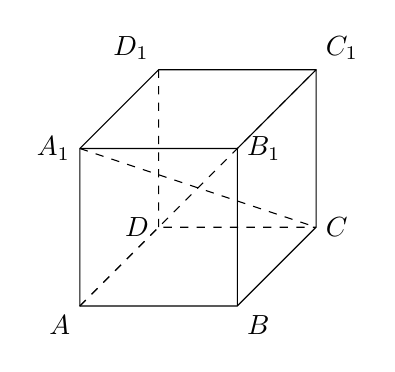
\begin{tikzpicture}
        \draw (0,0) node [below left] {$A$} coordinate (A) --++ (2,0) node [below right] {$B$} coordinate (B) --++ (45:{2*sqrt(2)/2}) node [right] {$C$} coordinate (C)
        --++ (0,2) node [above right] {$C_1$} coordinate (C1)
        --++ (-2,0) node [above left] {$D_1$} coordinate (D1) --++ (225:{2*sqrt(2)/2}) node [left] {$A_1$} coordinate (A1) -- cycle;
        \draw (A) ++ (2,2) node [right] {$B_1$} coordinate (B1) -- (B) (B1) --++ (45:{2*sqrt(2)/2}) (B1) --++ (-2,0);
        \draw [dashed] (A) --++ (45:{2*sqrt(2)/2}) node [left] {$D$} coordinate (D) --++ (2,0) (D) --++ (0,2);
        \draw [dashed] (A1) -- (C) (A) --(C1);
    \end{tikzpicture}
\end{center}
\item 椭圆的长轴长等于$m$, 短轴长等于$n$, 则此椭圆的内接矩形的面积的最大值为\blank{50}.

% 赋能44

\item 已知集合$A=\{1,2,3\}B=\{1,m\}$, 若$3-m\in A$, 则非零实数$m$的数值是\blank{50}.
\item 不等式$|1-x|>1$的解集是\blank{50}.
\item 若函数$f(x)=\sqrt{8-ax-2x^2}$是偶函数, 则该函数的定义域是\blank{50}.
\item 已知$\triangle ABC$的三内角$A,B,C$所对的边长分别为$a,b,c$, 若$a^2=b^2+c^2-2bc\sin A$, 则内角$A$的大小是\blank{50}.
\item 已知向量$\overrightarrow a$在向量$\overrightarrow b$方向上的投影为$-2$, 且$|\overrightarrow b|=3$, 则$\overrightarrow a\cdot \overrightarrow b$=\blank{50}(结果用数值表示).
\item 方程$\log_3(3 \cdot 2^x+5)-\log_3(4^x+1)=0$的解$x=$\blank{50}.
\item 已知函数$f(x)=\begin{vmatrix}
2\sin x & -\cos 2x  \\ 1  & \cos x  \end{vmatrix}$, 则函数$f(x)$的单调递增区间是\blank{50}.
\item 已知$\alpha$是实系数一元二次方程$x^2-(2m-1)x+m^2+1=0$的一个虚数根, 且$|\alpha|\le 2$, 则实数$m$的取值范围是\blank{50}.
\item 已知某市A社区$35$岁至$45$岁的居民有$450$人, $46$岁至$55$岁的居民有$750$人, $56$岁至$65$岁的居民有$900$人. 为了解该社区$35$岁至$65$岁居民的身体健康状况, 社区负责人采用分层抽样技术抽取若干人进行体检调查, 若从$46$岁至$55$岁的居民中随机抽取了$50$人, 试问这次抽样调查抽取的人数是\blank{50}人.
\item 将一枚质地均匀的硬币连续抛掷$5$次, 则恰好有$3$次出现正面向上的概率是\blank{50}(结果用数值表示).

% 赋能45

\item 函数$y=3\sin(2x+\dfrac{\pi}3)$的最小正周期T=\blank{50}.
\item 函数$y=\lg x$的反函数是\blank{50}.
\item 已知集合$P=\{x|(x+1)(x-3)<0\}$, $Q=\{x||x|>2\}$, 则$P\cap Q$=\blank{50}.
\item 函数$y=x+\dfrac9x$, $x\in (0,+\infty)$的最小值是\blank{50}.
\item 计算: $\displaystyle\lim_{n\to\infty}[\dfrac12+\dfrac14+\dfrac18+\cdots+(\dfrac12)^n]$=\blank{50}.
\item 记球$O_1$和$O_2$的半径、体积分别为$r_1$、$V_1$和$r_2$、$V_2$, 若$\dfrac{V_1}{V_2}=\dfrac8{27}$, 则$\dfrac{r_1}{r_2}=$\blank{50}.
\item 若某线性方程组对应的增广矩阵是$\begin{pmatrix} m & 4 & 2 \\ 1 & m & m \end{pmatrix}$, 且此方程组有唯一一组解, 则实数$m$的取值范围是\blank{50}.
\item 若一个布袋中有大小、质地相同的三个黑球和两个白球, 从中任取两个球, 则取出的两球中恰是一个白球和一个黑球的概率是\blank{50}.
\item $(1+2x)^n$的二项展开式中, 含$x^3$项的系数等于含$x$项的系数的$8$倍, 则正整数$n=$\blank{50}.
\item 平面上三条直线$x-2y+1=0$, $x-1=0$, $x+ky=0$, 如果这三条直线将平面划分为六个部分, 则实数$k$的取值组成的集合$A=$\blank{50}.

% 赋能46

\item 已知集合$A=\{1,3,5,7,9\}$, $B=\{0,1,2,3,4,5\}$, 则图中阴影部分集合用列举法表示的结果是\blank{50}.
\begin{center}
    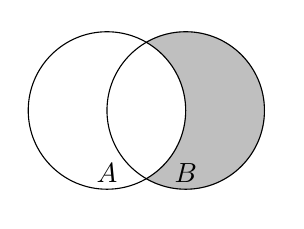
\begin{tikzpicture}
        \filldraw [color = lightgray] (0.5,{0.5*sqrt(3)}) arc (60:-60:1) arc (-120:120:1);
        \draw (0,0) circle (1);
        \draw (1,0) circle (1);
        \draw (0,-0.8) node {$A$};
        \draw (1,-0.8) node {$B$};
    \end{tikzpicture}
\end{center}
\item 若复数$z$满足$z(1-\mathrm{i})=2 \mathrm{i}$($\mathrm{i}$是虚数单位), 则$|z|=$\blank{50}.
\item 函数$y=\sqrt{\lg(x+2)}$的定义域为\blank{50}.
\item 在从$4$个字母$a$、$b$、$c$、$d$中任意选出$2$个不同字母的试验中, 其中含有字母$d$事件的概率是\blank{50}.
\item 如图的三个直角三角形是一个体积为$20\text{cm}^3$的几何体的三视图, 则$h=$\blank{50}.
\begin{center}
    \begin{tikzpicture}[>=latex]
        \draw (0,0) -- (2.5,0) -- (0,2) -- cycle;
        \draw (0,-0.1) -- (0,-0.3) (2.5,-0.1) -- (2.5,-0.3);
        \draw (1.25,-0.2) node {$5$};
        \draw [->] (1.05,-0.2) -- (0,-0.2);
        \draw [->] (1.45,-0.2) -- (2.5,-0.2);
        \draw (1.25,-0.5) node {主视图};
        \draw (-0.1,0) -- (-0.3,0) (-0.1,2) -- (-0.3,2);
        \draw (-0.2,1) node {$h$};
        \draw [->] (-0.2,0.8) -- (-0.2,0);
        \draw [->] (-0.2,1.2) -- (-0.2,2);
        \draw (3.5,0) -- (6.5,0) -- (3.5,2) -- cycle;
        \draw (3.5,-0.1) -- (3.5,-0.3) (6.5,-0.1) -- (6.5,-0.3);
        \draw (5,-0.2) node {$6$};
        \draw [->] (4.8,-0.2) -- (3.5,-0.2);
        \draw [->] (5.2,-0.2) -- (6.5,-0.2);
        \draw (5,-0.5) node {左视图};
        \draw (0,-1) -- (2.5,-1) -- (0,-4) -- cycle;
        \draw (1.25,-4.5) node {俯视图};
    \end{tikzpicture}
\end{center}
\item 如图, 以长方体$ABCD-A_1B_1C_1D_1$的顶点$D$为坐标原点, 过$D$的三条棱所在的直线为坐标轴, 建立空间直角坐标系, 若$\overrightarrow{DB_1}$的坐标为$(4,3,2)$, 则$\overrightarrow{BD_1}$的坐标为\blank{50}.
\begin{center}
    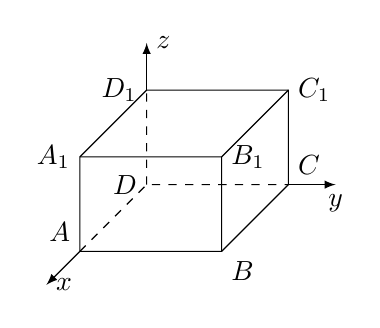
\begin{tikzpicture}[scale = 0.6, >=latex]
        \draw (0,0) node [above left] {$A$} coordinate (A) --++ (3,0) node [below right] {$B$} coordinate (B) --++ (45:{4/2}) node [above right] {$C$} coordinate (C)
        --++ (0,2) node [right] {$C_1$} coordinate (C1)
        --++ (-3,0) node [left] {$D_1$} coordinate (D1) --++ (225:{4/2}) node [left] {$A_1$} coordinate (A1) -- cycle;
        \draw (A) ++ (3,2) node [right] {$B_1$} coordinate (B1) -- (B) (B1) --++ (45:{4/2}) (B1) --++ (-3,0);
        \draw [dashed] (A) --++ (45:{4/2}) node [left] {$D$} coordinate (D) --++ (3,0) (D) --++ (0,2);
        \draw [->] (A) --++ (225:1) node [right] {$x$};
        \draw [->] (C) --++ (1,0) node [below] {$y$};
        \draw [->] (D1) --++ (0,1) node [right] {$z$};
    \end{tikzpicture}
\end{center}
\item 方程$\cos 2x=-\dfrac{\sqrt3}2$的解集为\blank{50}.
\item 已知抛物线的顶点在坐标原点, 焦点在$y$轴上, 抛物线上一点$M(a,-4) \ (a>0)$到焦点F的距离为$5$. 则该抛物线的标准方程为\blank{50}.
\item 已知等比数列$\{a_n\}$的前$n$项和为$S_n$($n\in \mathbf{N}*$), 且$\dfrac{S_6}{S_3}=-\dfrac{19}8$,$a_4-a_2=-\dfrac{15}8$, 则$a_3$的值为\blank{50}.
\item 在直角三角形$ABC$中, $\angle A=\dfrac{\pi}2$, $AB=3$, $AC=4$, $E$为三角形$ABC$内一点, 且$AE=\dfrac{\sqrt2}2$. 若$\overrightarrow{AE}=\lambda \overrightarrow{AB}+\mu \overrightarrow{AC}$, 则$3\lambda +4 \mu$的最大值等于\blank{50}.

% 赋能47

\item 双曲线$\dfrac{x^2}{a^2}-\dfrac{y^2}9=1 \ (a>0)$的渐近线方程为$3x\pm 2y=0$, 则$a=$\blank{50}.
\item 若二元一次方程组的增广矩阵是$\begin{pmatrix} 1 & 2 & c_1  \\ 3 & 4 & c_2 \end{pmatrix}$, 其解为$\begin{cases} x=10, \\ y=0, \end{cases}$ 则$c_1+c_2=$\blank{50}.
\item 设$m\in \mathbf{R}$, 若复数$(1+m\mathrm{i})(1+\mathrm{i})$在复平面内对应的点位于实轴上, 则$m=$\blank{50}.
\item 定义在$\mathbf{R}$上的函数$f(x)=2^x-1$的反函数为$y=f^{-1}(x)$, 则$f^{-1}(3)=$\blank{50}.
\item 直线$l$的参数方程为$\begin{cases}  x=1+t, \\ y=-1+2t, \end{cases}$($t$为参数), 则$l$的一个法向量为\blank{50}.
\item 已知数列$\{a_n\}$, 其通项公式为$a_n=3n+1$, $n\in \mathbf{N}^*$, $\{a_n\}$的前$n$项和为$S_n$, 则$\displaystyle\lim_{n\to\infty}\dfrac{S_n}{n\cdot {a_n}}=$\blank{50}.
\item 已知向量$\overrightarrow a$、$\overrightarrow b$的夹角为$60^{\circ}$, $|\overrightarrow a|=1$, $|\overrightarrow b|=2$, 若$(\overrightarrow a+2 \overrightarrow b)\perp (x\overrightarrow a-\overrightarrow b)$, 则实数$x$的值为\blank{50}.
\item 若球的表面积为$100 \pi$, 平面$\alpha$与球心的距离为$3$, 则平面$\alpha$截球所得的圆面面积为\blank{50}.
\item 若平面区域的点$(x,y)$满足不等式$\dfrac{|x|}k+\dfrac{|y|}4\le 1\ (k>0)$, 且$z=x+y$的最小值为$-5$, 则常数$k=$\blank{50}.
\item 若函数$f(x)={\log_a}(x^2-ax+1)\ (a>0, \ a\ne 1)$没有最小值, 则$a$的取值范围是\blank{50}.

% 赋能48

\item $\displaystyle\lim_{n\to \infty}\dfrac{2n+1}{n-1}=$\blank{50}.
\item 不等式$\dfrac x{x-1}<0$的解集为\blank{50}.
\item 已知$\{a_n\}$是等比数列, 它的前$n$项和为$S_n$, 且$a_3=4$, $a_4=-8$, 则$S_5=$\blank{50}.
\item 已知$f^{-1}(x)$是函数$f(x)=\log_2(x+1)$的反函数, 则$f^{-1}(2)=$\blank{50}.
\item $(\sqrt x+\dfrac1x)^9$二项展开式中的常数项为\blank{50}.
\item 椭圆$\begin{cases} x=2 \cos\theta, \\ y=\sqrt3\sin\theta  \end{cases}$($\theta$为参数)的右焦点为\blank{50}.
\item 满足约束条件$\begin{cases} x+2y\le 4, \\ 2x+y\le 3, \\ x\ge 0, \\ y\ge 0 \end{cases}$的目标函数$f=3x+2y$的最大值为\blank{50}.
\item 函数$f(x)=\cos^2 x+\dfrac{\sqrt3}2\sin 2x,\ x\in \mathbf{R}$的单调递增区间为\blank{50}.
\item 已知抛物线型拱桥的顶点距水面$2$米时, 量得水面宽为$8$米. 当水面下降$1$米后, 水面的宽为\blank{50}米.
\item 一个四面体的顶点在空间直角坐标系$O-xyz$中的坐标分别是$(0,0,0)$, $(1,0,1)$, $(0,1,1)$, $(1,1,0)$, 则该四面体的体积为\blank{50}.

% 赋能49

\item 抛物线$x^2=12y$的准线方程为\blank{50}.
\item 若函数$f(x)=\dfrac1{x-2m+1}$是奇函数, 则实数$m=$\blank{50}.
\item 若函数$f(x)=\sqrt{2x+3}$的反函数为$g(x)$, 则函数$g(x)$的零点为\blank{50}.
\item 书架上有上、中、下三册的《白话史记》和上、下两册的《古诗文鉴赏辞典》, 现将这五本书从左到右摆放在一起, 则中间位置摆放中册《白话史记》的不同摆放种数为\blank{50}(结果用数值表示).
\item 在锐角三角形$ABC$中, 角$A$、$B$、$C$的对边分别为$a$、$b$、$c$, 若$(b^2+c^2-a^2)\tan A=bc$, 则角$A$的大小为\blank{50}.
\item 若$(x^3-\dfrac1{x^2})^n$的展开式中含有非零常数项, 则正整数$n$的最小值为\blank{50}.
\item 某单位年初有两辆车参加某种事故保险, 对在当年内发生此种事故的每辆车, 单位均可获赔(假设每辆车最多只获一次赔偿). 设这两辆车在一年内发生此种事故的概率分别为$\dfrac1{20}$和$\dfrac1{21}$, 且各车是否发生事故相互独立, 则一年内该单位在此种保险中获赔的概率为\blank{50}(结果用最简分数表示).
\item 在平面直角坐标系$xOy$中, 直线$l$的参数方程为$\begin{cases} x=\dfrac{\sqrt2}2t-\sqrt2, \\ y=\dfrac{\sqrt2}4t, \end{cases}$($t$为参数), 椭圆$C$的参数方程为$\begin{cases} x=\cos \theta,  \\ y=\dfrac12\sin \theta,  \end{cases}$($\theta$为参数), 则直线$l$与椭圆$C$的公共点坐标为\blank{50}.
\item 设函数$f(x)=\log_m x$($m>0$且$m\ne 1$), 若$m$是等比数列$\{a_n\}$($n\in \mathbf{N}^*$)的公比, 且$f(a_2a_4a_6\cdots a_{2018})=7$, 则$f(a_1^2)+f(a_2^2)+f(a_3^2)+\cdots+f(a_{2018}^2)$的值为\blank{50}.
\item 设变量$x,y$满足条件$\begin{cases}  x-y\ge 0, \\ 2x+y\le 2, \\ y\ge 0, \\ x+y\le m, \end{cases}$ 若该条件表示的平面区域是三角形, 则实数$m$的取值范围是\blank{50}.

% 赋能50

\item 不等式$|x-3|<2$的解集为\blank{50}.
\item 若复数$z$满足$2 \overline z-3=1+5 \mathrm{i}$($\mathrm{i}$是虚数单位), 则$z=$\blank{50}.
\item 若$\sin\alpha =\dfrac13$, 则$\cos(\alpha -\dfrac{\pi}2)=$\blank{50}.
\item 已知两个不同向量$\overrightarrow{OA}=(1,m)$, $\overrightarrow{OB}=(m-1,2)$, 若$\overrightarrow{OA}\perp =\overrightarrow{AB}$, 则实数$m=$\blank{50}.
\item 在等比数列$\{a_n\}$中, 公比$q=2$, 前$n$项和为$S_n$, 若$S_5=1$, 则$S_{10}=$\blank{50}.
\item 若$x,y$满足$\begin{cases}x\le 2, \\ x-y+1\ge 0, \\ x+y-2\ge 0,\end{cases}$ 则$z=2x-y$的最小值为\blank{50}.
\item 如图所示, 一个圆柱的主视图和左视图都是边长为$1$的正方形,\blank{50}俯视图是一个直径为$1$的圆, 那么这个圆柱的体积为\blank{50}.
\begin{center}
    \begin{tikzpicture}
        \draw (0,0) rectangle (1.2,1.2) (1.8,0) rectangle (3,1.2);
        \draw (0.6,-0.3) node {主视图} (2.4,-0.3) node {左视图};
        \draw (0.6,-1.4) circle (0.6);
        \draw (0.6,-2.3) node {俯视图};
    \end{tikzpicture}
\end{center}
\item $(1+\dfrac1{x^2})(1+x)^6$展开式中$x^2$的系数为\blank{50}.
\item 已知$f(x)$是定义在$[-2,2]$上的奇函数, 当$x\in (0,2]$时,$f(x)=2^x-1$, 函数$g(x)=x^2-2x+m$. 如果对于任意的$x_1\in [-2,2]$, 总存在$x_2\in [-2,2]$, 使得$f(x_1)\le g(x_2)$, 则实数$m$的取值范围是\blank{50}.
\item 已知曲线$C:y=-\sqrt{9-x^2}$, 直线$l:y=2$, 若对于点$A(0,m)$, 存在$C$上的点$P$和$l$上的点$Q$, 使得$\overrightarrow{AP}+\overrightarrow{AQ}=\overrightarrow 0$, 则$m$取值范围是\blank{50}.

% 赋能51

\item 函数$y=\lg x-1$的零点是\blank{50}.
\item 计算:$\displaystyle\lim_{n\to\infty}\dfrac{2n}{4n+1}=$\blank{50}.
\item 若$(1+3x)^n$的二项展开式中$x^2$项的系数是$54$, 则$n=$\blank{50}.
\item 掷一颗均匀的骰子, 出现奇数点的概率为\blank{50}.
\item 若$x,y$满足$\begin{cases} x-y\ge 0, \\ x+y\le 2, \\ y\ge 0, \end{cases}$ 则目标函数$f=x+2y$的最大值为\blank{50}.
\item 若复数$z$满足$|z|=1$, 则$|z-\mathrm{i}|$的最大值是\blank{50}.
\item 若一个圆锥的主视图(如图所示)是边长为$3,3,2$的三角形, 则该圆锥的体积是\blank{50}.
\begin{center}
    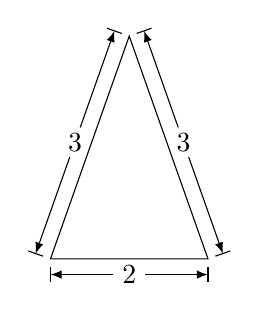
\begin{tikzpicture}[>=latex]
        \draw (-1,0) -- (1,0) -- (0,{2*sqrt(2)}) -- cycle;
        \draw (-1,-0.1) -- (-1,-0.3) (1,-0.1) -- (1,-0.3);
        \draw (0,-0.2) node {$2$};
        \draw [->] (-0.2,-0.2) -- (-1,-0.2);
        \draw [->] (0.2,-0.2) -- (1,-0.2);
        \draw (1,0) ++ ({asin(1/3)}:0.1) --++ ({asin(1/3)}:0.2);
        \draw (0,{2*sqrt(2)}) ++ ({asin(1/3)}:0.1) --++ ({asin(1/3)}:0.2);
        \draw [->] ($(1,0)!{1.3/3}!(0,{2*sqrt(2)})$) ++ ({asin(1/3)}:0.2) --++ ({-acos(1/3)}:1.3);
        \draw [->] ($(1,0)!{1.7/3}!(0,{2*sqrt(2)})$) ++ ({asin(1/3)}:0.2) --++ ({180-acos(1/3)}:1.3);
        \draw ($(1,0)!{0.5}!(0,{2*sqrt(2)})$) ++ ({asin(1/3)}:0.2) node {$3$};
        \draw (-1,0) ++ ({180-asin(1/3)}:0.1) --++ ({180-asin(1/3)}:0.2);
        \draw (0,{2*sqrt(2)}) ++ ({180-asin(1/3)}:0.1) --++ ({180-asin(1/3)}:0.2);
        \draw [->] ($(-1,0)!{1.3/3}!(0,{2*sqrt(2)})$) ++ ({180-asin(1/3)}:0.2) --++ ({180+acos(1/3)}:1.3);
        \draw [->] ($(-1,0)!{1.7/3}!(0,{2*sqrt(2)})$) ++ ({180-asin(1/3)}:0.2) --++ ({acos(1/3)}:1.3);
        \draw ($(-1,0)!{0.5}!(0,{2*sqrt(2)})$) ++ ({180-asin(1/3)}:0.2) node {$3$};
    \end{tikzpicture}
\end{center}
\item 若双曲线$\dfrac{x^2}3-\dfrac{16y^2}{p^2}=1\ (p>0)$的左焦点在抛物线$y^2=2px$的准线上, 则$p=$\blank{50}.
\item 若$\sin(x-y)\cos x-\cos(x-y)\sin x=\dfrac35$, 则$\tan 2y$的值为\blank{50}.
\item 若$\{a_n\}$为等比数列, $a_n>0$, 且$a_{2018}=\dfrac{\sqrt2}2$, 则$\dfrac1{a_{2017}}+\dfrac2{a_{2019}}$的最小值为\blank{50}.

% 赋能52

\item 已知集合$A=\{1,2,m\}$,$B=\{2,4\}$, 若$A\cup B=\{1,2,3,4\}$, 则实数$m=$\blank{50}.
\item$(x+\dfrac1x)^n$的展开式中的第$3$项为常数项, 则正整数$n=$\blank{50}.
\item 已知复数$z$满足${z^2}=4+3\mathrm{i}$($\mathrm{i}$为虚数单位), 则$|z|=$\blank{50}.
\item 已知平面直角坐标系$xOy$中动点$P(x,y)$到定点$(1,0)$的距离等于$P$到定直线$x=-1$的距离, 则点$P$的轨迹方程为\blank{50}.
\item 已知数列$\{a_n\}$是首项为$1$, 公差为$2$的等差数列,$S_n$是其前$n$项和, 则$\displaystyle\lim_{n\to\infty}\dfrac{S_n}{a_n^2}=$\blank{50}.
\item 设变量$x,y$满足条件$\begin{cases} x\ge 1, \\ x+y-4\le 0, \\  x-3y+4\le 0,  \end{cases}$ 则目标函数$z=3x-y$的最大值为\blank{50}.
\item 将圆心角为$\dfrac{2\pi}3$, 面积为$3\pi$的扇形围成一个圆锥的侧面, 则此圆锥的体积为\blank{50}.
\item 三棱锥$P-ABC$及其三视图中的主视图和左视图如图所示, 则棱$PB$的长为\blank{50}.
\begin{center}
    \begin{tikzpicture}[>=latex]
        \draw (0,0) node [right] {$C$} coordinate (C) -- (0,2) node [above] {$P$} coordinate (P) -- (-2,0) node [left] {$A$} coordinate (A);
        \draw (-1,0) ++ (-135:{sqrt(3)/2}) node [below] {$B$} coordinate (B) -- (A) (B) -- (C) (B) -- (P);
        \draw [dashed] (A) -- (C);
        \draw (2,0) -- (4,0) -- (4,2) -- cycle;
        \draw (3,0) -- (4,2);
        \draw (5,0) -- ({5+sqrt(3)},0) coordinate (D) -- (5,2) -- cycle;
        \draw (2,-0.1) -- (2,-0.3) (3,-0.1) -- (3,-0.3) (4,-0.1) -- (4,-0.3);
        \draw [->] (2.2,-0.2) -- (2,-0.2);
        \draw [->] (2.8,-0.2) -- (3,-0.2);
        \draw [->] (3.2,-0.2) -- (3,-0.2);
        \draw [->] (3.8,-0.2) -- (4,-0.2);
        \draw (2.5,-0.2) node {$2$} (3.5,-0.2) node {$2$};
        \draw (3,-0.7) node {主视图};
        \draw (5,-0.1) -- (5,-0.3) (D) ++ (0,-0.1) --++ (0,-0.2);
        \draw [->] ({5+sqrt(3)/2-0.4},-0.2) -- (5,-0.2);
        \draw [->] ({5+sqrt(3)/2+0.4},-0.2) -- ({5+sqrt(3)},-0.2);
        \draw ({5+sqrt(3)/2},-0.2) node {$2\sqrt{3}$};
        \draw ({5+sqrt(3)/2},-0.7) node {主视图};
        \draw (4.9,0) -- (4.7,0) (4.9,2) -- (4.7,2);
        \draw [->] (4.8,0.8) -- (4.8,0);
        \draw [->] (4.8,1.2) -- (4.8,2);
        \draw (4.8,1) node {$4$};
    \end{tikzpicture}
\end{center}
\item 某商场举行购物抽奖促销活动, 规定每位顾客从装有编号为$0$、$1$、$2$、$3$的四个相同小球的抽奖箱中, 每次取出一球记下编号后放回, 连续取两次, 若取出的两个小球编号相
加之和等于$6$, 则中一等奖, 等于$5$中二等奖, 等于$4$或$3$中三等奖. 则顾客抽奖中三等奖的概率为\blank{50}.
\item 已知函数$f(x)=\lg (\sqrt{x^2+1}+ax)$的定义域为$\mathbf{R}$, 则实数$a$的取值范围是\blank{50}.

% 赋能53

\item 已知全集$U=\mathbf{R}$,若集合$A=\{x|\dfrac x{x-1}>0\}$, 则$\complement_U A=$\blank{50}.
\item 已知复数$z$满足$z\cdot (1-\mathrm{i})=2\mathrm{i}$, 其中$\mathrm{i}$为虚数单位, 则$|z|=$\blank{50}.
\item 双曲线$2 x^2-y^2=6$的焦距为\blank{50}.
\item 已知$(ax+\dfrac1x)^6$二项展开式中的第五项系数为$\dfrac{15}2$, 则正实数$a$\blank{50}.
\item 方程$\log_2(9^x+7)=2+\log_2(3^x+1)$的解为\blank{50}.
\item 已知函数$f(x)=\dfrac{3x+1}{x+a}\ (a\ne \dfrac13)$的图像与它的反函数的图像重合, 则实数$a$的值为\blank{50}.
\item 在$\triangle ABC$中, 边$a,b,c$所对角分别为$A,B,C$, 若$\begin{vmatrix} a & \sin (\dfrac{\pi}2+B)  \\ b & \cos A  \end{vmatrix}=0$, 则$\triangle ABC$的形状为\blank{50}.
\item 若某几何体的三视图(单位:$\text{cm}$)如图所示, 则此几何体的体积是\blank{50}$\text{cm}^3$.
\begin{center}
    \begin{tikzpicture}[>=latex,scale = 0.7]
        \draw (1,0) -- (2,0) -- (2,3) -- (3,3) -- (3,4) -- (0,4) -- (0,3) -- (1,3) -- cycle;
        \draw (5,0) -- (8,0) -- (8,4) -- (5,4) -- cycle (5,3) -- (8,3);
        \draw (0,-1) -- (0,-4) -- (3,-4) -- (3,-1) -- cycle;
        \draw [dashed] (1,-1) -- (1,-4) (2,-1) -- (2,-4);
        \draw (1.5,-4.5) node {俯视图} (1.5,-0.5) node {主视图} (6.5,-0.5) node {俯视图};
        \draw (3.1,-4) -- (3.3,-4) (3.1,-1) -- (3.3,-1);
        \draw [->] (3.2,-2.1) -- (3.2,-1);
        \draw [->] (3.2,-2.9) -- (3.2,-4);
        \draw (3.2,-2.5) node {$3$};
        \draw (5,4.1) -- (5,4.3) (8,4.1) -- (8,4.3);
        \draw [->] (6.1,4.2) -- (5,4.2);
        \draw [->] (6.9,4.2) -- (8,4.2);
        \draw (6.5,4.2) node {$3$};
        \draw (0,4.1) -- (0,4.3) (1,4.1) -- (1,4.3) (2,4.1) -- (2,4.3) (3,4.1) -- (3,4.3);
        \draw [->] (0.3,4.2) -- (0,4.2);
        \draw [->] (0.7,4.2) -- (1,4.2);
        \draw (0.5,4.2) node {$1$};
        \draw [->] (1.3,4.2) -- (1,4.2);
        \draw [->] (1.7,4.2) -- (2,4.2);
        \draw (1.5,4.2) node {$1$};
        \draw [->] (2.3,4.2) -- (2,4.2);
        \draw [->] (2.7,4.2) -- (3,4.2);
        \draw (2.5,4.2) node {$1$};
        \draw (3.1,4) -- (3.3,4) (3.1,3) -- (3.3,3) (3.1,0) -- (3.3,0);
        \draw [->] (3.2,1.1) -- (3.2,0);
        \draw [->] (3.2,1.9) -- (3.2,3);
        \draw (3.2,1.5) node {$3$};
        \draw [->] (3.2,3.2) -- (3.2,3);
        \draw [->] (3.2,3.8) -- (3.2,4);
        \draw (3.2,3.5) node {$1$};
    \end{tikzpicture}
\end{center}
\item 已知四面体$ABCD$中, $AB=CD=2$, $E$, $F$分别为$BC$, $AD$的中点, 且异面直线$AB$与$CD$所成的角为$\dfrac{\pi}3$, 则$EF$=\blank{50}.
\item 设$m,n$分别为连续两次投掷骰子得到的点数, 且向量$\overrightarrow a=(m,n)$,$\overrightarrow b=(1,-1)$, 则$\overrightarrow a$与$\overrightarrow b$的夹角为锐角的概率是\blank{50}.
\item 已知数列$\{a_n\}$的通项公式为$a_n={(-1)}^n\cdot n+2^n, \ n\in \mathbf{N}^*$, 则这个数列的前$2n$项和$S_{2n}=$\blank{50}.

% 赋能54

\item 设集合$A=\{x||x|<2,\ x\in \mathbf{R}\}$, $B=\{x|x^2-4x+3\ge 0, \ x\in \mathbf{R}\}$, 则$A\cap B=$\blank{50}.
\item 已知$\mathrm{i}$为虚数单位, 复数$z$满足$\dfrac{1-z}{1+z}=\mathrm{i}$, 则$|z|=$\blank{50}.
\item 设$a>0$且$a\ne 1$, 若函数$f(x)=a^{x-1}+2$的反函数的图像经过定点$P$, 则点$P$的坐标是\blank{50}.
\item 计算: $\displaystyle\lim_{n\to\infty}\dfrac{\mathrm{P}_n^2+\mathrm{C}_n^2}{(n+1)^2}=$\blank{50}.
\item 在平面直角坐标系内, 直线$l:2x+y-2=0$, 将$l$与两条坐标轴围成的封闭图形绕$y$轴旋转一周, 所得几何体的体积为\blank{50}.
\item 已知$\sin 2\theta +\sin\theta =0$,$\theta \in (\dfrac{\pi}2,\pi)$, 则$\tan 2\theta =$\blank{50}.
\item 设定义在$\mathbf{R}$上的奇函数$y=f(x)$, 当$x>0$时, $f(x)=2^x-4$, 则不等式$f(x)\le 0$的解集是\blank{50}.
\item 在平面直角坐标系$xOy$中, 有一定点$A(1,1)$, 若线段$OA$的垂直平分线过抛物线$C:y^2=2px \ (p>0)$的焦点, 则抛物线$C$的方程为\blank{50}.
\item 曲线$\begin{cases} x=1-\dfrac{\sqrt5}5 t, \\ y=-1+\dfrac{2\sqrt5}5t, \end{cases}$($t$为参数)与曲线$\begin{cases} x=\sin \theta \cdot \cos \theta, \\ y=\sin \theta +\cos \theta,  \end{cases}$($\theta$为参数)的公共点的坐标为\blank{50}.
\item 记$(2x+\dfrac1x)^n \ (n\in \mathbf{N}^*$)的展开式中第$m$项的系数为$b_m$, 若$b_3=2b_4$, 则$n=$\blank{50}.
\item 已知各项均为正数的数列$\{a_n\}$满足$\sqrt{a_1}+\sqrt{a_2}+\cdots+\sqrt{a_n}=n^2+3n$($n\in \mathbf{N}^*$), 则$\dfrac{a_1}2+\dfrac{a_2}3+\cdots \dfrac{a_n}{n+1}=$\blank{50}.

% 赋能55

\item 函数$f(x)=\dfrac{\sqrt{x+2}}{x-1}$的定义域为\blank{50}.
\item 已知线性方程组的增广矩阵为$\begin{pmatrix} 1 & -1  & 3  \\ a & 3 & 4 \end{pmatrix}$, 若该线性方程组的解为$\begin{pmatrix} -1 \\ 2\end{pmatrix}$, 则实数$a=$\blank{50}.
\item 计算$\displaystyle\lim_{n\to\infty}\dfrac{1+2+3+\cdots +n}{n^2+1}=$\blank{50}.
\item 若向量$\overrightarrow a$、$\overrightarrow b$满足$|\overrightarrow a|=1$, $|\overrightarrow b|=2$, 且$\overrightarrow a$与$\overrightarrow b$的夹角为$\dfrac{\pi}3$, 则$|\overrightarrow a+\overrightarrow b|=$\blank{50}.
\item 若复数$z_1=3+4\mathrm{i}$, $z_2=1-2\mathrm{i},$ 其中$\mathrm{i}$是虚数单位, 则复数$\dfrac{|z_1|}{\mathrm{i}}+\overline{z_2}$的虚部为\blank{50}.
\item $(\dfrac1x-\sqrt x)^6$的展开式中, 常数项为\blank{50}.
\item 已知$\triangle  ABC$的内角$A$、$B$、$C$所对应边的长度分别为$a$、$b$、$c$, 若$\begin{vmatrix}a & c \\ c & a\end{vmatrix} = \begin{vmatrix}-b & -a \\ b & b\end{vmatrix}$, 则角$C$的大小是\blank{50}.
\item 已知等比数列$\{a_n\}$的各项均为正数, 且满足:$a_1a_7=4$, 则数列$\{\log_2a_n\}$的前$7$项之和为\blank{50}.
\item 已知双曲线$x^2-\dfrac{y^2}4=1$的右焦点为$F$, 过点$F$且平行于双曲线的一条渐近线的直线与双曲线交于点$P$, $M$在直线$PF$上, 且满足$\overrightarrow{OM}\cdot \overrightarrow{PF}=0$, 则$\dfrac{|\overrightarrow{PM}|}{|\overrightarrow{PF}|}=$\blank{50}.
\item 现有$5$位教师要带$3$个班级外出参加志愿者服务, 要求每个班级至多两位老师带队, 且教师甲、乙不能单独带队, 则不同的带队方案有\blank{50}(用数字作答).

% 赋能56

\item 抛物线$y^2=4x$的焦点坐标是\blank{50}.
\item 若集合$A=\{x|3x+1>0\}$, $B=\{x||x-1|<2\}$, 则$A\cap B$=\blank{50}.
\item 若$\overrightarrow d=(3,2)$是直线$l$的一个方向向量, 则$l$的倾斜角的大小为\blank{50}(结果用反三角函数值表示).
\item 若复数$z$满足$\dfrac{1-\mathrm{i}}z=-\mathrm{i}$, 其中$\mathrm{i}$为虚数单位, 则$z=$\blank{50}.
\item 求值:$\begin{vmatrix}\arcsin\dfrac{\sqrt3}2 & 2  \\ \arctan\dfrac{\sqrt3}3 & 3  \end{vmatrix}$=\blank{50}弧度.
\item 已知$\overrightarrow{AB}=3\overrightarrow{AP}$, 设$\overrightarrow{BP}=\lambda \overrightarrow{PA}$, 则实数$\lambda=$\blank{50}.
\item 函数$y=\sqrt{x^2+2}+\dfrac1{\sqrt{x^2+2}}$的最小值为\blank{50}.
\item 试写出$(x-\dfrac1x)^7$展开式中系数最大的项\blank{50}.
\item 已知三个球的表面积之比是$1:2:3$, 则这三个球的体积之比为\blank{50}.
\item 已知实数$x,y$满足$\begin{cases}x+y\ge 2, \\ x-y\le 2, \\ 0 \le y\le 3, \end{cases}$ 则目标函数$z=-\dfrac32x-y$的最大值为\blank{50}.
\item 若不等式$x^2-5x+6<0$的解集为$(a,b)$, 则$\displaystyle\lim_{n\to\infty}\dfrac{a^n-2b^n}{3a^n-4b^n}=$\blank{50}.
\item 从集合$A=\{1,2,3,4,5,6,7,8,9,10\}$中任取两个数, 欲使取到的一个数大于$k$, 另一个数小于$k$(其中$k\in A$)的概率是$\dfrac25$, 则$k=$\blank{50}.

% 赋能57

\item 设函数$f(x)=a^x+a^{-x}  \ (a>0, \ a\ne 1)$, 且$f(1)=3$, 则$f(0)+f(1)+f(2)$的值是\blank{50}.
\item 已知集合$A=\{x||x-2|<a\}$, $B=\{x|x^2-2x-3<0\}$, 若$B\subseteq A$, 则实数$a$的取值范围是\blank{50}.
\item 如果复数$z$满足$|z|=1$且$z^2=a+b\mathrm{i}$, 其中$a,b\in \mathbf{R}$, 则$a+b$的最大值是\blank{50}.
\item 已知$x,y$满足$\begin{cases}
   x-y+5 \ge 0, \\ x+y\ge 0, \\ x\le 3, \end{cases}$ 若使得$z=ax+y$取最大值的点$(x,y)$有无数个, 则$a$的值等于\blank{50}.
\item 在直角坐标系$xOy$中, 已知三点$A(a,1),B(2,b),C(3,4)$, 若向量$\overrightarrow{OA}$, $\overrightarrow{OB}$在向量$\overrightarrow{OC}$方向上的投影相同, 则$3a-4b$的值是\blank{50}.
\item 已知$F_1,F_2$是椭圆$C:\dfrac{x^2}{a^2}+\dfrac{y^2}{b^2}=1\ (a>b>0)$的两个焦点, $P$为椭圆上一点, 且$\overrightarrow{PF_1}\perp \overrightarrow{PF_2}$, 若$\triangle PF_1F_2$的面积为$9$, 则$b=$\blank{50}.
\item$\triangle ABC$中,$a,b,c$分别是$\angle A,\angle B,\angle C$的对边且$ac+c^2=b^2-a^2$, 若$\triangle ABC$最大边长是$\sqrt7$且$\sin C=2\sin A$, 则$\triangle ABC$最小边的边长为\blank{50}.
\item 设等差数列$\{a_n\}$的公差为$d$, 若$a_1,a_2,a_3,a_4,a_5,a_6,a_7$的方差为$1$, 则$d$=\blank{50}.
\item 已知函数$f(x)=\begin{cases} \cos \dfrac{\pi x}2, & |x|\le 1,  \\ x^2-1, & |x|>1,  \end{cases}$ 则关于$x$的方程$f^2(x)-3f(x)+2=0$的实根的个数是\blank{50}个.


% 赋能58

\item 设集合$M=\{x|x^2=x\}$, $N=\{x|\log_2 x\le 0\}$, 则$M\cup N=$\blank{50}.
\item 已知虚数$1+2\mathrm{i}$是方程$x^2+ax+b=0 (a\,b\in \mathbf{R})$的一个根, 则$a+b=$\blank{50}.
\item 在报名的$5$名男生和$4$名女生中, 选取$5$人参加志愿者服务, 要求男、女生都有, 则不同的选取方式的种数为\blank{50}(结果用数值表示).
\item 已知复数$z$在复平面上对应的点在曲线$y=\dfrac 2 x$上运动, 则$|z|$的最小值等于\blank{50}.
\item 在正项等比数列$\{a_n\}$中, $a_1a_3=1$, $a_2+a_3=\dfrac43$, 则$\displaystyle\lim_{n\to\infty}(a_1+a_2+\cdots +a_n)=$\blank{50}.
\item 已知$f(x)=2 \sin \omega x\ (\omega >0)$在$[0,\dfrac\pi 3]$单调递增, 则实数$\omega$的最大值为\blank{50}.
\item 若行列式$\begin{vmatrix}   1 & 2 & 4 \\   \cos (\pi +x) & 2 & 0 \\   -1 & 1 & 6 \end{vmatrix}$中的元素$4$的代数余子式的值等于$\dfrac32$, 则实数$x$的取值集合为\blank{50}.
\item 若二项式$(2x-\dfrac1{\sqrt x})^n$展开式中的第$5$项为常数项, 则展开式中各项的二项式系数之和为\blank{50}.
\item 已知$A$、$B$是球$O$的球面上两点, $\angle AOB=90^\circ$, $C$为该球面上的动点, 若三棱锥$O-ABC$体积的最大值为$\dfrac{32}{3}$, 则球$O$的表面积为\blank{50}.
\begin{center}
    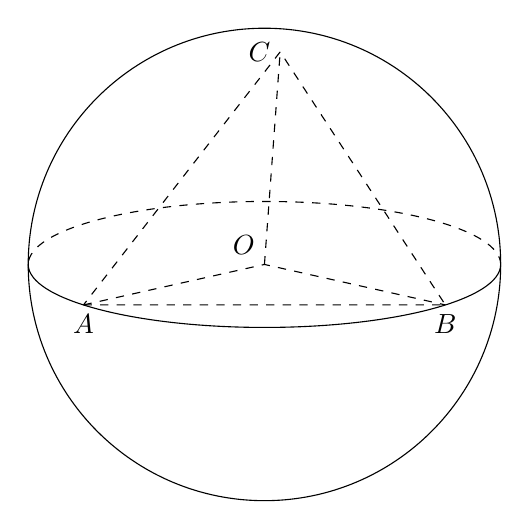
\begin{tikzpicture}
        \draw (0,0) circle (3);
        \draw (-3,0) arc (180:360:3 and 0.8);
        \draw [dashed] (3,0) arc (0:180:3 and 0.8);
        \draw ({3*cos(-140)},{0.8*sin(-140)}) coordinate (A) node [below] {$A$};
        \draw ({3*cos(-40)},{0.8*sin(-40)}) coordinate (B) node [below] {$B$};
        \draw (0.2,2.7) coordinate (C) node [left] {$C$};
        \draw (0,0) coordinate (O) node [above left] {$O$};
        \draw [dashed] (A) -- (B) -- (C) -- cycle;
        \draw [dashed] (A) -- (O) -- (B) (O) -- (C);
    \end{tikzpicture}
\end{center}
\item 如图, $A$、$B$为椭圆$\dfrac{x^2}{a^2}+\dfrac{y^2}{b^2}=1 \ (a>b>0)$的两个顶点, 过椭圆的右焦点$F$作$x$轴的垂线, 与其交于点$C$. 若$AB\parallel OC$($O$为坐标原点), 则直线$AB$的斜率为\blank{50}.
\begin{center}
    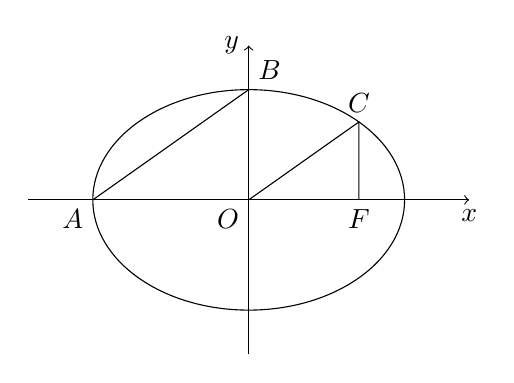
\begin{tikzpicture}[scale = 1.4]
        \draw [->] (-2,0) -- (2,0) node [below] {$x$};
        \draw [->] (0,-1.4) -- (0,1.4) node [left] {$y$};
        \draw (0,0) node [below left] {$O$};
        \draw (0,0) ellipse ({sqrt(2)} and 1);
        \draw (1,0) node [below] {$F$} -- (1,{sqrt(2)/2}) node [above] {$C$} -- (0,0);
        \draw ({-sqrt(2)},0) node [below left] {$A$} -- (0,1) node [above right] {$B$};
    \end{tikzpicture}
\end{center}
\item 若经过抛物线 $y^2=4x$焦点的直线$l$与圆$(x-4)^2+y^2=4$相切, 则直线$l$的方程为\blank{50}.

% 赋能59

\item 若集合$A=\{x|y=\sqrt{x-1},\ x\in \mathbf{R}\}$, $B=\{x||x|\le 1,\ x\in \mathbf{R}\}$, 则$A\cap B=$\blank{50}.
\item 若函数$f(x)=1+\dfrac1x$($x>0$)的反函数为$f^{-1}(x)$, 则不等式$f^{-1}(x)>2$的解集为\blank{50}.
\item 若$\sin \alpha =\dfrac35$且$\alpha$是第二象限角, 则$\tan(\alpha -\dfrac\pi 4)=$\blank{50}.
\item 若函数$f(x)$是定义在$\mathbf{R}$上的奇函数, 且满足$f(x+2)=-f(x)$, 则$f(2016)=$\blank{50}.
\item 在$(x^3-\dfrac1x)^8$的展开式中, 其常数项的值为\blank{50}.
\item 若函数$f(x)=\sin 2x$, $g(x)=f(x+\dfrac\pi 6)$, 则函数$g(x)$的单调递增区间为\blank{50}.
\item 设$P$是曲线$\begin{cases} x=\dfrac{\sqrt2}2\sec \theta, \\ y=\tan \theta \end{cases}$($\theta $为参数)上的一动点, $O$为坐标原点, $M$为线段$OP$的中点, 则点$M$的轨迹的普通方程为\blank{50}.
\item 不等式组$\begin{cases} x\le 3, \\ x+y\ge 0, \\ x-y+2 \ge 0 \end{cases}$所表示的区域的面积为\blank{50}.
\item 若函数$f(x)=\log _5 x$($x>0$), 则方程$f(x+1)+f(x-3)=1$的解$x=$\blank{50}.
\item 如图所示, 三个边长为$2$的等边三角形有一条边在同一直线上, 边$B_3C_3$上有$10$个不同的点$P_1,P_2,\cdots,P_{10}$, 记$M_i=\overrightarrow{AB_2}\cdot \overrightarrow{AP_i}$($i=1,2,\cdots,10$), 则$M_1+M_2+\cdots+M_{10}=$\blank{50}.
\begin{center}
    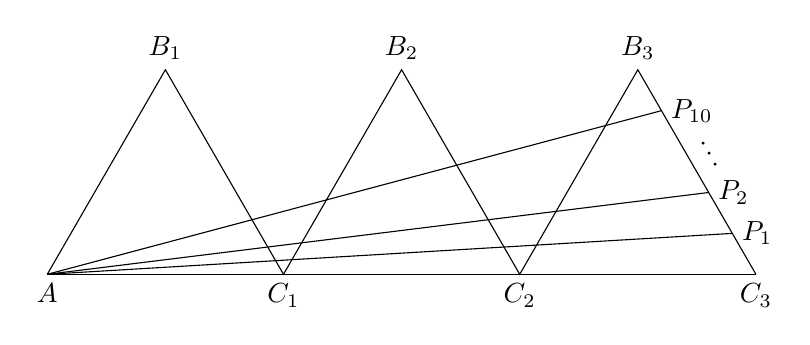
\begin{tikzpicture}[scale = 3]
        \draw (0,0) node [below] {$A$} -- (1,0) node [below] {$C_1$} -- (2,0) node [below] {$C_2$} -- (3,0) node [below] {$C_3$};
        \draw (3,0) -- (2.5,{sqrt(3)/2}) node [above] {$B_3$} -- (2,0) -- (1.5,{sqrt(3)/2}) node [above] {$B_2$} -- (1,0) -- (0.5,{sqrt(3)/2}) node [above] {$B_1$} -- (0,0);
        \draw ($(3,0)!0.2!(2.5,{sqrt(3)/2})$) coordinate (P1) node [right] {$P_1$} -- (0,0);
        \draw ($(3,0)!0.4!(2.5,{sqrt(3)/2})$) coordinate (P2) node [right] {$P_2$} -- (0,0);
        \draw ($(3,0)!0.8!(2.5,{sqrt(3)/2})$) coordinate (P3) node [right] {$P_{10}$} -- (0,0);
        \draw ($(3,0)!0.6!(2.5,{sqrt(3)/2})$) node [right] {\rotatebox{120}{$\cdots$}};
    \end{tikzpicture}
\end{center}

% 赋能60

\item 已知全集$U=\mathbf{R}$, $A=\{x|x^2-2x<0\}$, $B=\{x|x\ge 1\}$, 则$A\cap \complement_U B=$\blank{50}.
\item 若函数$y=\cos ^2 \omega x$($\omega >0$)的最小正周期是$\pi$, 则$\omega=$\blank{50}.
\item 圆$C:x^2+y^2-2x-4y+4=0$的圆心到直线$3x+4y+4=0$的距离$d=$\blank{50}.
\item 已知圆锥的母线长为$5\text{cm}$, 侧面积为$15 \pi \text{cm}^2$, 则此圆锥的体积为\blank{50}$\text{cm}^2$.
\item 已知$x,y\in \mathbf{R}^+$, 且满足$\dfrac x3+\dfrac y4=1$, 则$xy$的最大值为\blank{50}.
\item 已知双曲线$\dfrac{x^2}{a^2}-\dfrac{y^2}{b^2}=1 \ (a>0,\ b>0)$的一条渐近线方程是$y=\sqrt3x$, 它的一个焦点与抛物线$y^2=16x$的焦点相同, 则双曲线的标准方程为\blank{50}.
\item 已知函数$f(x)=\begin{cases}2^x +a, & x\ge 0, \\ x^2-ax, & x<0.\end{cases}$ 若$f(x)$的最小值是$a$, 则$a=$\blank{50}.
\item 从$6$名男医生和$3$名女医生中选出$5$人组成一个医疗小组, 若这个小组中必须男女医生都有, 共有\blank{50}种不同的组建方案(结果用数值表示).
\item 若数列$\{a_n\}$是首项为$1$, 公比为$a-\dfrac32$的无穷等比数列, 且$\{a_n\}$各项的和为$a$, 则$a$的值是\blank{50}.
\item 设$a\ne 0$, $n$是大于$1$的自然数, $(1+\dfrac xa)^n$的展开式为$a_0+a_1x+a_2x^2+\cdots+a_nx^n$. 若$a_1=3$, $a_2=4$, 则$a=$\blank{50}.
\item 矩形$ABCD$中, $AB=2$, $AD=1$, $P$为矩形内部一点, 且$AP=1$. 若$\overrightarrow{AP}=\lambda \overrightarrow{AB}+\mu \overrightarrow{AD} \ (\lambda,\ \mu \in \mathbf{R})$, 则$2 \lambda +\sqrt3\mu$的最大值是\blank{50}.

% 赋能61

\item 函数$y=\log_3 (x-1)$的定义域是\blank{50}.
\item 集合$A=\{x|x^2-3x<0\}$, $B=\{x||x|<2\}$, 则$A\cup B$等于\blank{50}.
\item 若复数$\dfrac{1+\mathrm{i}}{1-\mathrm{i}}+\dfrac12b$($\mathrm{i}$为虚数单位)的实部与虚部相等, 则实数$b$的值为\blank{50}.
\item 已知函数$f(x)=\begin{vmatrix}   {\log _3}x & 1  \\   2 & 1  \\\end{vmatrix}$, 则$f^{-1}(0)=$\blank{50}.
\item 若一个圆锥的母线长是底面半径的$3$倍, 则该圆锥的侧面积是底面积的\blank{50}倍.
\item 平面向量$\overrightarrow a$与$\overrightarrow b$的夹角为$60^\circ$, $|\overrightarrow a|=1$, $\overrightarrow b=(3,0)$, 则$|2 \overrightarrow a+\overrightarrow b|=$\blank{50}.
\item 已知$\triangle ABC$的周长为$4$, 且$\sin A+\sin B=3 \sin C$, 则$AB$边的长为\blank{50}.
\item 若$a_n$为$(1+x)^n$的展开式中的$x^2$项的系数, 则$\displaystyle\lim_{n\to\infty}\dfrac{2a_n}{n^2+1}=$\blank{50}.
\item 若$m>0$, $n>0$, $m+n=1$, 且$\dfrac t m+\dfrac 1 n$($t>0$)的最小值为$9$, 则$t=$\blank{50}.
\item 若以$x$轴正方向为始边, 曲线上的点与圆心的连线为终边的角$\theta$为参数, 则圆$x^2+y^2-2x=0$的参数方程为\blank{50}.
\item 若$AB$是圆$x^2+(y-3)^2=1$的任意一条直径, $O$为坐标原点, 则$\overrightarrow{OA}\cdot \overrightarrow{OB}$的值为\blank{50}.

% 赋能62

\item 已知集合$A=\{-1,3,2m-1\}$, 集合$B=\{3,m^2\}$. 若$B\subseteq A$, 则实数$m=$\blank{50}.
\item 计算: $\displaystyle\lim_{n\to\infty}\dfrac{3^n+1}{3^{n+1}+2^n}=$\blank{50}.
\item 函数$f(x)=\sqrt[3]x+1$的反函数$f^{-1}(x)=$\blank{50}.
\item 函数$f(x)=(\sin x-\cos x)^2$的最小正周期为\blank{50}.
\item 直线$x+2y-1=0$与直线$y=1$的夹角大小为\blank{50}(结果用反三角函数值表示).
\item 已知菱形$ABCD$, 若$|\overrightarrow{AB}|=1$, $A=\dfrac\pi 3$, 则向量$\overrightarrow{AC}$在$\overrightarrow{AB}$上的投影为\blank{50}.
\item 已知一个凸多面体的平面展开图由两个正六边形和六个正方形构成, 如图所示, 若该凸多面体所有棱长均为$1$, 则其体积$V=$\blank{50}.
\begin{center}
    \begin{tikzpicture}[scale = 0.6]
        \draw (0,0) -- (6,0) (0,1) -- (6,1);
        \foreach \i in {0,1,...,6}{\draw (\i,0) -- (\i,1);};
        \draw (1,1) --++ (60:1) --++ (120:1) --++ (180:1) --++ (240:1) --++ (300:1); 
        \draw (6,0) --++ (-60:1) --++ (-120:1) --++ (-180:1) --++ (-240:1) --++ (-300:1);
    \end{tikzpicture}
\end{center}
\item 已知函数$f(x)={x^3}+\lg (\sqrt{x^2+1}+x)$, 若$f(x)$的定义域中的$a$、$b$满足$f(-a)+f(-b)-3=f(a)+f(b)+3$, 则$f(a)+f(b)=$\blank{50}.
\item 数列$\{a_n\}$中, 若$a_1=3$, $\sqrt{a_{n+1}}=a_n$($n\in \mathbf{N}^*$), 则数列$\{a_n\}$的通项公式$a_n=$\blank{50}.
\item 在代数式$(4x^2-2x-5)(1+\dfrac1{x^2})^5$的展开式中, 常数等于\blank{50}.
\item 满足约束条件$|x|+2|y|\le 2 $的目标函数$z=y-x$的最大值是\blank{50}.
% 赋能63

\item 若$\mathrm{i}(b\mathrm{i}+1)$是纯虚数, $\mathrm{i}$是虚数单位, 则实数$b=$\blank{50}.
\item 函数$y=\sqrt{2^x-1}$的定义域是\blank{50}(用区间表示).
\item 已知$\triangle ABC$中, $|\overrightarrow{AB}|=2 $,  $|\overrightarrow{AC}|=3 $, $\overrightarrow{AB}\cdot \overrightarrow{AC}<0$, 且$\triangle ABC$的面积为$\dfrac32$, 则$\angle BAC=$\blank{50}.
\item 双曲线$4 x^2-y^2=1$的一条渐近线与直线$tx+y+1=0$垂直, 则$t=$\blank{50}.
\item 已知抛物线上一点$M(x_0,2 \sqrt3)$, 则点$M$到抛物线焦点的距离为\blank{50}.
\item 无穷等比数列首项为$1$,公比为$q \ (q>0)$, 前$n$项和为$S_n$, 若$\displaystyle\lim_{n\to\infty}S_n=2$, 则$q=$\blank{50}.
\item 在一个水平放置的底面半径为$\sqrt 3$的圆柱形量杯中装有适量的水, 现放入一个半径为$R$的实心铁球, 球完全浸没于水中且无水溢出, 若水面高度恰好上升$R$, 则$R$=\blank{50}.
\item 在平面直角坐标系$xOy$中, 将点$A(2,1)$绕原点$O$逆时针旋转$\dfrac\pi 4$到点$B$, 若直线$OB$的倾斜角为$\alpha$, 则$\cos \alpha$的值为\blank{50}.
\item 已知函数$f(x)=2^x-a\cdot 2^{-x}$的反函数是$f^{-1}(x)$, $f^{-1}(x)$在定义域上是奇函数, 则正实数$a=$\blank{50}.
\item 已知$x\ge 1$, $y\ge 0$, 集合$A=\{(x,y)|x+y\le 4\}$, $B=\{(x,y)|x-y+t=0\}$. 如果$A\cap B\ne \varphi$,则$t$的取值范围是\blank{50}.
\item 如图, 一个空间几何体的主视图、左视图、俯视图均为全等的等腰直角三角形, 如果直角三角形的直角边长都为$1$, 那么这个几何体的表面积为\blank{50}.
\begin{center}
    \begin{tikzpicture}
        \draw (0,2) -- (2,0) -- (0,0) -- cycle;
        \draw (1,0) node [below] {主视图};
        \draw (3,0) -- (5,0) -- (3,2) -- cycle;
        \draw (4,0) node [below] {左视图};
        \draw (0,-1) -- (2,-1) -- (0,-3) -- cycle;
        \draw (1,-3) node [below] {俯视图};
    \end{tikzpicture}
\end{center}

% 赋能64

\item 已知全集$U=\mathbf{R}$, 集合$A=\{x|(x-1)(x-4)\le 0\}$, 则集合$A$的补集$\complement_UA=$\blank{50}.
\item 指数方程$4^x-6 \times 2^x-16=0$的解是\blank{50}.
\item 已知无穷等比数列$\{a_n\}$的首项$a_1=18$, 公比$q=-\dfrac12$, 则无穷等比数列$\{a_n\}$各项的和是\blank{50}.
\item 函数$y=\cos 2x, \ x\in [0,\pi]$的递增区间为\blank{50}.
\item 抛物线$y^2=x$上一点$M$到焦点的距离为$1$, 则点M的横坐标是\blank{50}.
\item 一盒中装有$12$个同样大小的球, 其中$5$个红球, $4$个黑球, $2$个白球, $1$个绿球. 从中随机取出$1$个球, 则取出的$1$个球是红球或黑球或白球的概率为\blank{50}.
\item 关于$\theta$的函数$f(\theta)=\cos^2\theta-2x\cos\theta-1$的最大值记为$M(x)$, 则$M(x)$的解析式为\blank{50}.
\item 如图所示, 是一个由圆柱和球组成的几何体的三视图, 若$a=2$, $b=3$, 则该几何体的体积等于\blank{50}.
\begin{center}
    \begin{tikzpicture}[>=latex,scale = 0.6]
        \draw (0,1) circle (1);
        \draw (-1,-0.1) -- (-1,-0.3) (1,-0.1) -- (1,-0.3);
        \draw [->] (-0.2,-0.2) -- (-1,-0.2);
        \draw [->] (0.2,-0.2) -- (1,-0.2);
        \draw (0,-0.2) node {$a$};
        \draw (1.1,0) -- (1.3,0) (1.1,2) -- (1.3,2);
        \draw [->] (1.2,0.8) -- (1.2,0);
        \draw [->] (1.2,1.2) -- (1.2,2);
        \draw (1.2,1) node {$a$};
        \draw (0,-1) node {俯视图};
        \draw (-1,3.5) rectangle (1,6.5) (0,7.5) circle (1);
        \draw (-1,3.4) -- (-1,3.2) (1,3.4) -- (1,3.2);
        \draw [->] (-0.2,3.3) -- (-1,3.3);
        \draw [->] (0.2,3.3) -- (1,3.3);
        \draw (0,3.3) node {$a$};
        \draw (1.1,3.5) -- (1.3,3.5) (1.1,6.5) -- (1.3,6.5);
        \draw [->] (1.2,4.6) -- (1.2,3.5);
        \draw [->] (1.2,5.4) -- (1.2,6.5);
        \draw (1.2,5) node {$b$};
        \draw (0,2.5) node {主视图};
        \draw (3,3.5) rectangle (5,6.5) (4,7.5) circle (1);
        \draw (3,3.4) -- (3,3.2) (5,3.4) -- (5,3.2);
        \draw [->] (3.8,3.3) -- (3,3.3);
        \draw [->] (4.2,3.3) -- (5,3.3);
        \draw (4,3.3) node {$a$};
        \draw (5.1,3.5) -- (5.3,3.5) (5.1,6.5) -- (5.3,6.5);
        \draw [->] (5.2,4.6) -- (5.2,3.5);
        \draw [->] (5.2,5.4) -- (5.2,6.5);
        \draw (5.2,5) node {$b$};
        \draw (4,2.5) node {左视图};
    \end{tikzpicture}
\end{center}
\item 已知双曲线$x^2-\dfrac{y^2}{m^2}=1 \ (m>0)$的渐近线与圆$x^2+(y+2)^2=1$没有公共点, 则该双曲线的焦距的取值范围为\blank{50}.
\item 已知$\triangle ABC$外接圆的半径为$2$, 圆心为$O$, 且$\overrightarrow{AB}+\overrightarrow{AC}=2 \overrightarrow{AO}$, $|\overrightarrow{AB}|=|\overrightarrow{AO}|$, 则$\overrightarrow{CA}\cdot \overrightarrow{CB}=$\blank{50}.
\item 若不等式组$\begin{cases} x\ge 0, \\ x+3y\ge 4, \\  3x+y\le 4 \end{cases}$所表示的平面区域被直线$y=kx+\dfrac 43$分为面积相等的两部分, 则$k$的值是\blank{50}.
\end{enumerate}

\end{document}